% Workshop-style paper for the BlueDot state-dependence study.
% Build: pdflatex main && bibtex main && pdflatex main && pdflatex main
%
% Every number in this document was read from a verified run artifact in
% results/runs/bluedot-final-test/. Nothing here is estimated, rounded up, or reconstructed.
% See ../REPORT.md for the long-form version and the exact verification command.

\documentclass{article}

\usepackage[margin=1in]{geometry}
\usepackage{graphicx}
\usepackage{booktabs}
\usepackage{amsmath}
\usepackage{amssymb}
\usepackage{natbib}
\usepackage{hyperref}

\hypersetup{colorlinks=true, linkcolor=black, citecolor=black, urlcolor=blue}

\title{A Precommitted Benchmark for Activation-Intervention Forecasting:\\
A Null Test of Prompt-Specific Hidden-State Features\\
in Gemma 3 1B}

\author{Jacob Ortiz}

\date{July 2026}

\begin{document}

\maketitle

\begin{abstract}
We present a precommitted benchmark for forecasting the effect of an activation intervention before
it is applied, and a first application that returns a null. The benchmark asks a specific question:
given a complete numerical description of an intervention, does adding the prompt, the model's clean
output distribution, or the model's own hidden state improve prediction of what that intervention
will do? On \texttt{google/gemma-3-1b-it} at a pinned revision we add a fixed unit direction, scaled
by a single global strength chosen by preregistered calibration, to the layer-13 residual stream at
the final prompt token, and measure the shift in the margin around the model's own clean preferred
answer. The intervention family is fixed: eight directions and two signs, so 16 distinct signed
interventions, applied to every prompt at every stage. Three ridge regressions are fitted on 96
training prompts and frozen, then scored on 32 held-out prompts: intervention-only, a
visible-information baseline adding the prompt and clean logits, and a state-conditioned bilinear
model adding a 16-component PCA of the true hidden state and its interaction with the intervention.
A matched wrong-state condition substitutes another prompt's state without refitting. All 512
prompt-level forecasts, each covering all 17 candidates, were sealed under salted hashes before any
final-test intervention ran. Both preregistered comparisons are null: visible minus true-state MAE
is $-0.013725$, 95\% interval $[-0.025723, 0.00003]$; matched wrong-state minus true-state MAE is
$0.005172$, 95\% interval $[-0.003081, 0.013412]$; both cross zero over 10{,}000 paired bootstrap
resamples across 32 prompt groups. The lowest point-estimate MAE belongs to the intervention-only
ridge ($0.318821$, against $0.321518$ visible, $0.335244$ true-state, and $0.340416$ matched
wrong-state). An important limitation is that training and test share the intervention family, so
no method was asked to generalize to an unseen direction. The result illustrates why
intervention-level baselines, prompt-specificity controls, and forecast-before-outcome verification
are important when evaluating claims of privileged access to model internals.
\end{abstract}

\section{Introduction}

A recurring intuition in interpretability is that a model's internal state contains information
about its own computation that an external observer cannot get from the outside. This paper tests a
deliberately narrow, mechanical version of that intuition.

Take a small instruction-tuned model answering a four-choice science question. At one layer, at the
final prompt token, add a fixed unit vector to the residual stream and let the forward pass finish.
Measure how far the margin around the model's own clean preferred answer moved. Then try to
\emph{predict} that number in advance, for an intervention that has not been applied yet.

Two predictors get the same job and the same complete numerical description of the intervention.
Only one of them also sees the model's hidden state for that prompt. If the state-conditioned
predictor wins, the residual stream carried something about the intervention's consequences that
the visible channel did not. If it does not, then under this setup no improvement from state access
was detected, which is weaker than showing there is none.

Two things about the framing. First, this is an \emph{external state-information audit}: the
predictors are ridge regressions that we fit and control. A ridge regression reading a residual
stream is a readout, not a report, and the model is never asked about itself. Nothing here tests
introspection, self-awareness, faithful verbal reasoning, hidden goals, or deployment readiness.
Second, a win alone would not be enough, since a state-conditioned model might improve simply by
having more parameters and more variance to exploit. What makes a win meaningful is substituting a
\emph{different} prompt's state and checking that performance collapses.

We preregistered both hypotheses, the target, the intervention strength grid, the permitted layers,
the pass conditions, the aggregation unit, the number of bootstrap resamples, the seed, and the
decision rule, all before any outcome existed:

\begin{itemize}
  \item \textbf{H-BD1.} The state-conditioned ridge achieves lower prompt-aggregated mean absolute
        error than the visible-information ridge.
  \item \textbf{H-BD2.} That advantage depends on the state belonging to the prompt being
        predicted, so substituting a matched wrong state raises the error.
\end{itemize}

Neither is supported. The state-conditioned model's point-estimate MAE is higher than both
baselines', and substituting a matched wrong state does not degrade it detectably.

Our contribution is primarily the benchmark: a precommitted task for forecasting causal
intervention effects, an intervention-only and a visible-information baseline that are hard to
beat, a matched wrong-state specificity control, forecast-before-outcome ordering that is provable
from artifacts rather than asserted, and a standalone replay bundle. The null is the first
application, not the headline. Its scope is narrow by construction: on this fixed family of 16
signed interventions, neither the tested prompt features nor the tested hidden-state representation
produced a detected forecasting improvement over intervention-level information. That does not
imply that hidden states carry no useful information, that the tested methods are equivalent, that
the state-conditioned model is established to be worse, or that the finding extends to unseen
interventions, other models, other layers, other tasks, or other state readouts.

\section{Related Work}

This study responds to work asking whether models have privileged access to facts about their own
computation. \citet{li2025explain} fine-tune language models to describe, in natural language, the
information their features encode, the causal structure of their internal activations, and the
influence of input tokens on their outputs, and report that a model explaining its own computations
generally outperforms a different model explaining them, even a more capable one. That
self-versus-other advantage motivates our question, but our experiment tests something considerably
weaker and structurally different: whether an external linear readout of one hidden state helps
predict the numerical effect of a residual-stream perturbation. It does not test whether a model can
explain its own computation, and it is not a replication of their released explainer results.

Methodologically this is a probing study with a control condition, and the probing literature
supplies the cautions it operates under. \citet{hewitt2019control} argue that probe accuracy is
uninterpretable without a control that separates information in the representation from capacity in
the probe; our matched wrong-state condition serves a related purpose, holding the probe and the
intervention fixed while destroying only the correspondence between state and prompt, though it is
not identical to a control task in their sense. \citet{belinkov2022probing} sets out why successful
prediction from a representation does not by itself establish that the model uses that information
in the relevant way, which is why we describe this as a readout rather than a report.
\citet{voita2020mdl} show that probe complexity and sample efficiency shape what probe performance
can support at all, a concern that applies directly here: our state-conditioned model carries 327
features fitted on 96 prompts.

The intervention mechanism comes from activation engineering: adding a direction to the residual
stream at inference time to control the output \citep{turner2023activation}. We follow the mechanism
but not its recipe for choosing directions. Where activation addition derives a steering vector from
a contrast pair of prompts, our eight directions come from the pinned output embedding and a seeded
random orthogonal complement, so a real steer and a matched control can be published to the
predictors under identical metadata.

The precommitment protocol adapts preregistration practice, whose purpose is to keep prediction
distinct from postdiction by fixing the question and the analysis plan before outcomes are observed
\citep{nosek2018preregistration}, to a setting where the ``outcome'' is a set of forward passes the
experimenter can run at will. That is why the protocol here is enforced by salted hashes and refusal
conditions in code rather than by a filed document.

We want to be precise about what this study is \emph{not}. It is not a replication of any released
explainer result: different model, different intervention family, different target, and predictors
we fitted ourselves, which are external ridge regressions rather than a model trained to verbalize
anything about itself. A direct reproduction using the released Qwen3-8B and Llama-3.1-8B explainer
checkpoints and training code \citep{transluce2025introspectiveinterp} would be a separate
experiment, and we did not attempt one.

The task is ARC-Challenge \citep{clark2018arc}, the model is Gemma 3 1B instruction-tuned
\citep{gemmateam2025gemma3, gemma3_1b_it}, and the implementation uses Transformers
\citep{wolf2020transformers}, PyTorch \citep{paszke2019pytorch}, scikit-learn
\citep{pedregosa2011scikit}, and NumPy \citep{harris2020numpy}.

\section{Methods}

\subsection{Setup}

The model is \texttt{google/gemma-3-1b-it} at revision
\texttt{dcc83ea841ab6100d6b47a070329e1ba4cf78752}, run on CPU in float32 with hidden dimension
1152. Model revisions are typed to reject moving pointers such as \texttt{main}.

The task is ARC-Challenge rendered as four-choice items under a single neutral prompt wrapper. A
frozen split assigns 168 prompts to four disjoint roles: 8 smoke, 32 calibration, 96 training, and
32 final test. It is drawn by a seeded permutation of 256 eligible ARC group ids, disjoint by item
and by group, and selection never reads correctness, confidence, logits, or hidden states, so the
split cannot have been chosen to suit a result.

The target is $\Delta_{\text{margin}}$ (\texttt{delta\_clean\_top\_margin}): the shift in the margin
around the model's \emph{own} clean preferred answer, held fixed after the intervention. Clean
correctness against the dataset key does not enter the measurement.

The intervention family is eight unit vectors: four centered answer-token unembedding directions
and four seeded random controls orthogonal to their span and to each other. With both signs plus a
no-op this gives 17 candidates per prompt.

\paragraph{What the intervention block can and cannot represent.} Because the intervention strength
is global and the same eight directions are used at every stage, the intervention block takes only
16 distinct non-no-op values in the entire study. The intervention-only ridge therefore emits one
prediction per signed direction and cannot condition on the prompt: it functions as a regularized
table of direction-specific average effects. This is the correct reading of the frozen design
rather than a defect discovered afterwards, and it sharpens what the comparisons test. The central
question is whether visible prompt information or prompt-specific hidden-state information explains
residual variation beyond those direction-level effects. It also means no method is asked to
generalize to an intervention it has not seen; all of them interpolate across prompts within a known
family.

What is withheld from the predictors is the \emph{semantic label}, not the vector. A real steer
and a matched random control are published with identical metadata and an opaque identifier, while
every method receives $P^{\top} v$, a fixed 16-dimensional projection of the vector actually added.
A predictor can therefore tell directions apart numerically and could in principle recover structure
correlated with construction role; what it cannot do is read the mechanism off the metadata and
discount the controls without consulting anything else.

The strength is a single \emph{global} alpha, $\alpha = r \cdot \tilde{n}$, where $\tilde{n}$ is
the median clean state norm over the calibration prompts and $r$ is the selected ratio. It is
deliberately not prompt-relative: if $\alpha$ depended on $\lVert h_{\text{prompt}} \rVert$, the
visible-information baseline would silently receive the prompt's own state norm and the central
comparison would be contaminated at the source.

\subsection{Preregistered calibration}

The calibration plan fixed the target, five ratios $\{0.02, 0.05, 0.10, 0.20, 0.40\}$, two permitted
layers (13 primary, 20 fallback), and six pass conditions before any number existed. The run
captured all clean states first, took the median norm as the reference, derived one alpha per ratio,
then swept all 16 signed directions and a shared no-op per prompt: 2{,}624 forwards, zero failures.
The selector takes the \emph{smallest} passing ratio in preregistered order, never the largest
effect, because choosing the stimulus by its outcome would make the comparison circular. Ratio
$0.02$ was the smallest passing strength (Table~\ref{tab:calibration}), giving
$\alpha = 106.87158268272867$; ratios $0.10$, $0.20$, and $0.40$ each failed on exactly one
condition, the p95 ceiling of $4.0$, at $5.22$, $11.08$, and $23.58$. Layer 13 produced a usable
ratio, so the layer-20 fallback was prohibited.

\begin{table}[htbp]
\centering
\small
\begin{tabular}{lr}
\toprule
Quantity at ratio 0.02, layer 13 & Value \\
\midrule
Non-no-op observations & 512 \\
Failures & 0 \\
Answer flips & 19 (3.71\%) \\
Observations with $|\Delta_{\text{margin}}| \geq 0.10$ & 394 / 512 \\
Median $|\Delta_{\text{margin}}|$ & 0.23317 \\
p95 $|\Delta_{\text{margin}}|$ & 0.91024 \\
Maximum $|$no-op target$|$ & exactly 0 \\
\bottomrule
\end{tabular}
\caption{The selected calibration setting. Ratio 0.05 also passed every condition; 0.02 was
selected because it is smaller, not because it scored better.}
\label{tab:calibration}
\end{table}

One calibration diagnostic constrains what a positive result could have meant. At the selected
strength, the four answer-token directions and the four random controls flipped the answer at
nearly the same rate: 10/256 versus 9/256 (3.91\% versus 3.52\%), and 22/768 versus 23/768 in
training. The answer-token directions are built from the unembedding, but at this strength they do
not behave like a privileged causal handle relative to norm-matched random directions.

\subsection{Predictors}

Every method receives the same intervention block $P^{\top} v$, where $v$ is the 1152-dimensional
intervention vector and $P$ is a fixed $1152 \times 16$ projection generated once from the master
seed, never fitted, and cited by hash from every forecast. The four blocks are:

\begin{itemize}
  \item \textbf{Intervention} (16): $P^{\top} v$, identical across every method.
  \item \textbf{Visible} (39): four centered clean answer logits, clean top margin, clean entropy,
        prompt token count, and 32 train-only TF-IDF plus truncated-SVD components of the prompt
        text. Contains no state-derived quantity.
  \item \textbf{State} (16): train-only PCA of the 1152-dimensional clean residual stream.
  \item \textbf{Interaction} (256): flattened outer product of the state and intervention blocks.
\end{itemize}

\paragraph{Why a bilinear interaction.} For an intervention $\delta$ applied to the state $h$, and
writing $m$ for the map from the layer-13 state to the clean top margin, the induced change is
approximately
\begin{equation*}
  \Delta m \;\approx\; \nabla m(h)^{\top} \delta ,
\end{equation*}
a linear functional of $\delta$ whose coefficients depend on $h$. We do not claim $\delta$ is
infinitesimal or that this approximation is exact at the calibrated strength; it is a guide to what
each feature set can express. The intervention block alone can fit only one such functional shared
by every prompt, that is, an average local response. The state-by-intervention block is an attempt
to let the response vary with the state: with state features $S$ and intervention features $I$, the
256 interaction weights parameterize a bilinear form $S^{\top} W I$, a low-rank approximation to how
local sensitivity changes across prompts. A null is therefore consistent with several distinct
situations the design cannot separate: local sensitivity may vary little across these prompts, the
variation may lie outside the 16-dimensional state and intervention projections, 96 prompts may be
too few to fit 256 interaction weights, or the ridge penalty may suppress a weak state-dependent
signal.

Ridge penalties were selected by six-fold grouped cross-validation over a fixed eight-point grid,
grouping by prompt (Table~\ref{tab:predictors}). The TF-IDF vectorizer, the SVD, the state PCA, and
the feature standardizer were fitted on the 96 training prompts only, over 1{,}536 rows; each fit
record carries the prompt ids it saw and a hash of that list, and cannot be constructed with a fit
role other than \texttt{training}. Two model-free diagnostics locate the floor: a \textbf{constant}
predictor emitting the training mean, and a \textbf{prompt lexical} predictor regressing on
bag-of-words features that never sees the intervention.

\begin{table}[htbp]
\centering
\small
\begin{tabular}{lrrr}
\toprule
Method & Dim. & Ridge $\lambda$ & Training-fold CV MAE \\
\midrule
Intervention-only ridge   &  16 &   100 & 0.338847 \\
Visible-information ridge &  55 &  1000 & 0.343321 \\
State bilinear ridge      & 327 & 10000 & 0.361691 \\
\bottomrule
\end{tabular}
\caption{Frozen predictors. The state bilinear model selected the largest penalty on the grid, a
grid-edge selection recorded as such: cross-validation wanted more regularization than the grid
offered.}
\label{tab:predictors}
\end{table}

\subsection{Specificity controls}

For each final-test prompt a donor state is chosen deterministically from the other 31: the nearest
by clean top margin and clean entropy, restricted to donors sharing the model's clean preferred
label. No prompt is its own donor, all 32 matches share the preferred label, and the median margin
distance to a donor is $0.27$. Matching makes the substitution hard to detect for the wrong reason,
since an arbitrary donor would differ in gross, easily separable ways. Ten further conditions apply
seeded derangements over the 32 prompts. Substitution changes \emph{only} the state and interaction
blocks; the intervention and visible blocks are byte-identical to the true-state condition, so any
difference is attributable to the state alone.

\subsection{Precommitment and resolution}

Every forecast was produced before any final-test outcome existed. The 32 final-test prompts first
went through a clean-only stage that applied no intervention; predictors and transforms were then
frozen, and 512 commitment records were written, one for each of 16 method-and-condition
combinations on each of 32 prompts. \textbf{Each record covers all 17 candidates for its prompt},
so the 512 records seal $512 \times 17 = 8{,}704$ candidate-level predictions; nothing was committed
at one granularity and scored at another. Each commitment is a salted hash, which protects the
ordering rather than the content: the salts are published in the reveals after resolution, because
a commitment hash cannot be checked without them. The resolver verified that every commitment
predated every outcome artifact, and the published bundle lets a third party repeat that check
without a model. Table~\ref{tab:integrity} reports what resolution measured; the full refusal
conditions, key structure, and storage layout are documented with the artifacts.

\begin{table}[htbp]
\centering
\small
\begin{tabular}{lr}
\toprule
Integrity check & Result \\
\midrule
Prompts & 32 / 32 \\
Intervened forwards & 544 / 544 \\
Failures & 0 \\
Commitments verified and revealed & 512 / 512 \\
Every commitment predates every outcome & yes \\
All integrity checks passed exactly & yes \\
Realized answer flips & 6 \\
\bottomrule
\end{tabular}
\caption{Final-test integrity, as measured at resolution. No clean forward ran during resolution:
clean logits and states were reused from the clean stage, so every delta is measured against exactly
the baseline the forecasts were made against. Every stored target was independently recomputed from
its own logits.}
\label{tab:integrity}
\end{table}

\subsection{Analysis}

Absolute errors are averaged \emph{within each prompt first}, over that prompt's 16 non-no-op
interventions, and then across the 32 prompts. This was fixed in advance because the 16
interventions on one prompt share a question and a state.

Both primary comparisons use 10{,}000 paired bootstrap resamples over the 32 prompt groups with the
frozen seed 1394099119. Each replicate draws one set of prompt groups and evaluates both methods on
that same set. The decision rule, fixed before the data existed: a comparison supports its
hypothesis only if the 95\% paired interval excludes zero in the hypothesized direction. An interval
crossing zero is reported as no detected difference, never as a trend.

\section{Results}

\begin{figure}[htbp]
\centering
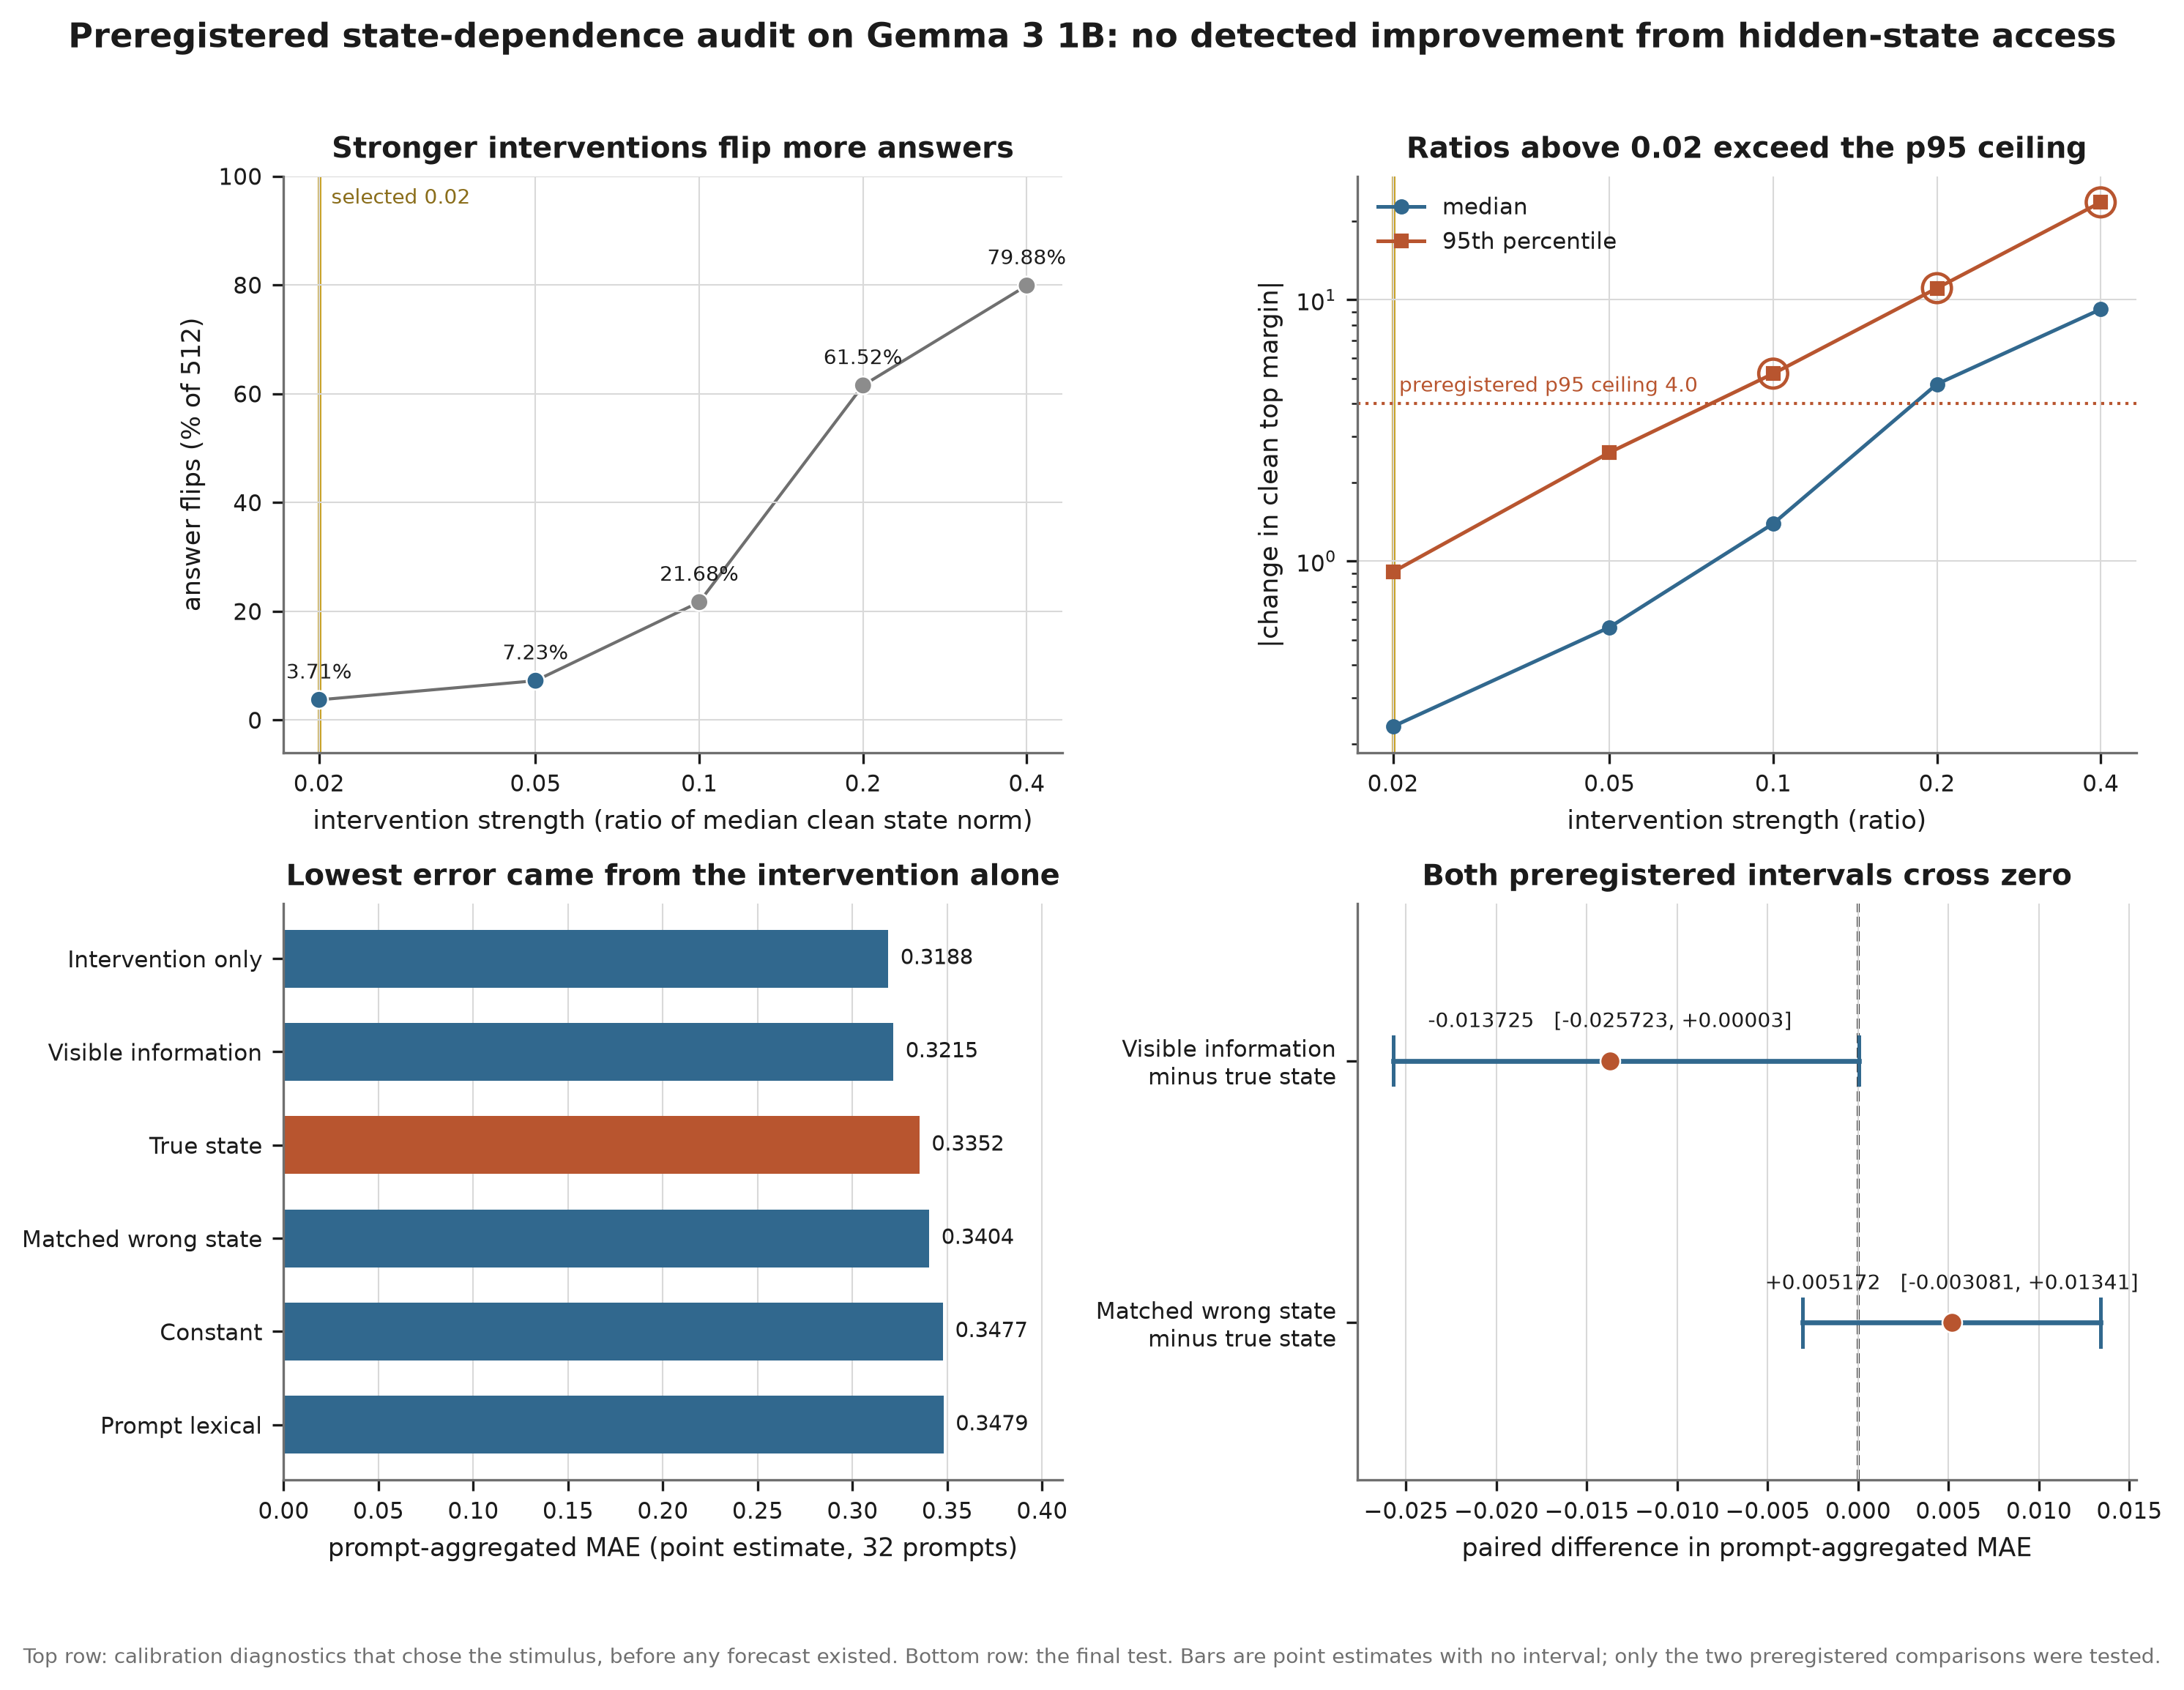
\includegraphics[width=0.86\textwidth]{figures/study_overview.png}
\caption{The benchmark on one page. Top: the calibration diagnostics that fixed the stimulus before
any forecast existed, with the selected ratio and the preregistered p95 ceiling marked. Bottom: the
final test, as point-estimate error by method and as the two preregistered paired comparisons. Bars
carry no interval; only the two comparisons were tested.}
\label{fig:overview}
\end{figure}

Scoring used the sealed forecasts and the verified outcomes. Nothing was fitted, refitted, tuned, or
dropped. Table~\ref{tab:main} gives the main result; the lower panels of Figure~\ref{fig:overview}
show it graphically.

\begin{table}[htbp]
\centering
\small
\begin{tabular}{lrrrrr}
\toprule
Method & MAE & RMSE & Sign acc. & Spearman & Top-effect acc. \\
\midrule
Intervention-only ridge   & \textbf{0.318821} & 0.402262 & 0.630859 & 0.357776 & 0.34375 \\
Visible-information ridge & 0.321518 & 0.404996 & 0.630859 & 0.353763 & 0.34375 \\
True-state bilinear ridge & 0.335244 & 0.421573 & 0.580078 & 0.296136 & 0.12500 \\
Matched wrong-state ridge & 0.340416 & 0.426767 & 0.566406 & 0.183944 & 0.06250 \\
Constant                  & 0.347682 & 0.433596 & 0.560547 & 0.056294 & 0.12500 \\
Prompt lexical            & 0.347937 & 0.434402 & 0.552734 & 0.057504 & 0.12500 \\
\bottomrule
\end{tabular}
\caption{Final-test performance, 32 prompts and 512 signed pairs per row. All values are point
estimates; only the two comparisons in Section~\ref{sec:primary} carry intervals, so differences
between rows that are not tested there are not established as differences.}
\label{tab:main}
\end{table}

\subsection{Primary comparisons}
\label{sec:primary}

\paragraph{H-BD1: visible minus true-state MAE.}
Point estimate $-0.013725$, 95\% interval $[-0.025723, 0.00003]$. The interval crosses zero, so
\textbf{H-BD1 is not supported}. The point estimate also has the wrong sign for the hypothesis: the
visible model's point-estimate MAE is the lower of the two. The upper endpoint is small but
positive, not zero; we write it as $0.00003$ rather than $0.0000$ so that it is not read as an
interval that terminates exactly at zero.

\paragraph{H-BD2: matched wrong-state minus true-state MAE.}
Point estimate $0.005172$, with a 95\% interval of $[-0.003081, 0.013412]$. The interval crosses
zero, so \textbf{H-BD2 is not supported}.

Both are shown in Figure~\ref{fig:primary}. Under the preregistered decision rule these are null
results: no improvement from state access was detected under this setup, and no dependence on the
state being the right one was detected. We do not describe either as a trend, and neither is a
demonstration of equivalence. An interval that crosses zero is consistent with a small true effect
in either direction, and with 32 prompt groups this design has limited power to resolve one.

\begin{figure}[htbp]
\centering
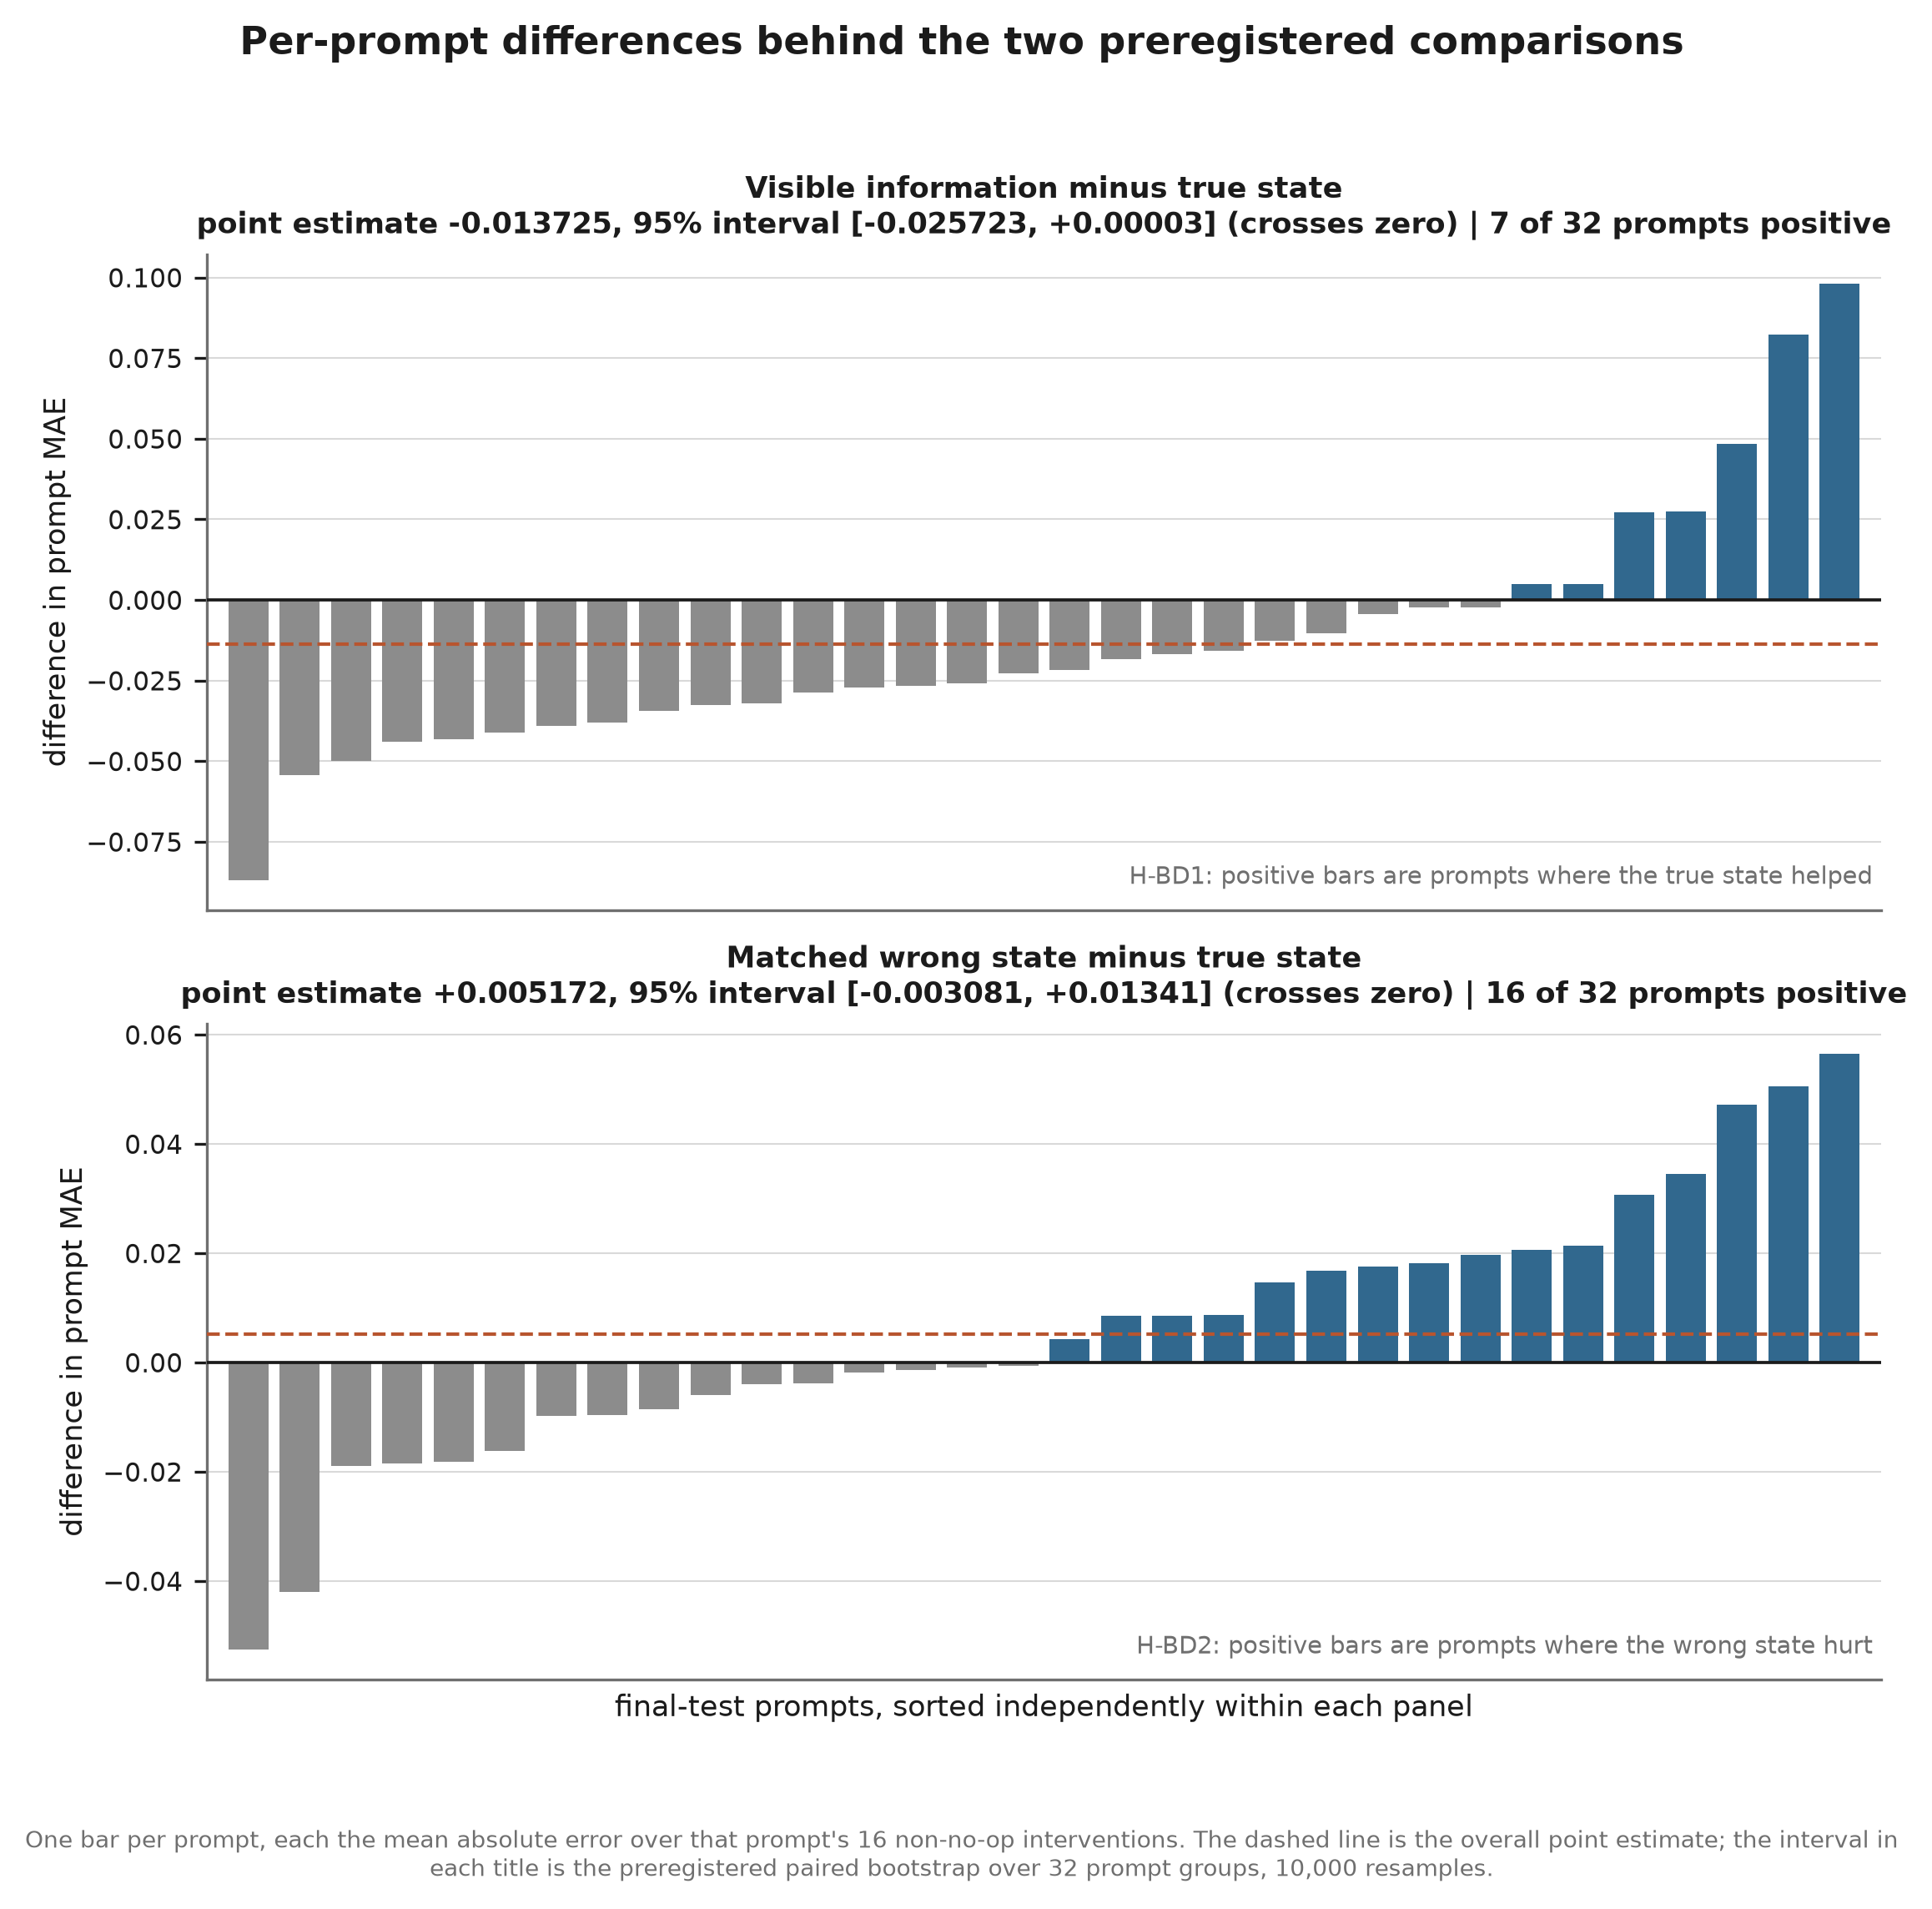
\includegraphics[width=0.80\textwidth]{figures/per_prompt_differences.png}
\caption{The two preregistered comparisons and the per-prompt differences behind them. Each
bar is one final-test prompt's mean absolute error over its 16 non-no-op interventions, sorted
independently within each panel; the dashed line is the overall point estimate and each title
carries the preregistered interval. Both cross zero. The per-prompt view is included because a
paired difference of this size is easy to over-read from a single summary number.}
\label{fig:primary}
\end{figure}

\subsection{Shuffled-state band and Brier score}

The ten seeded derangements, scored without refitting, give MAE mean $0.339221$, median $0.339280$,
minimum $0.335087$, maximum $0.342696$. The true-state MAE of $0.335244$ falls at the lower edge of
this range and the matched wrong-state MAE of $0.340416$ falls inside it.

This band is \textbf{descriptive only}. It is the spread of ten point estimates over ten seeds, not
a null distribution, not a confidence interval, and not a test: the derangements were not drawn to
support an inference, no interval was preregistered for them, and ten values give no useful tail.
It is reported because a reader should be able to see where the true-state score sits relative to
deliberately wrong states, and it is consistent with the H-BD2 result, but no conclusion rests on
it.

The Brier score is omitted. Only 6 answer flips occurred across all 512 final-test interventions,
below the preregistered floor of 20. The floor is enforced in the record type: a summary carrying a
Brier score over fewer than 20 flips cannot be constructed.

\subsection{Interpretation}

The result is best interpreted as a statement about residual prompt-specific signal after accounting
for a fixed intervention family. Direction-specific average effects captured much of the
forecastable structure. Under this design, neither the prompt and clean-output features nor the
tested PCA-bilinear state representation produced a detected improvement over those
intervention-level effects.

\paragraph{Supported.} Intervention identity carried useful predictive signal: every method
improves on the constant baseline, and the intervention-only ridge had the lowest point-estimate
MAE. The tested state representation produced no detected incremental improvement over the visible
baseline, and matched wrong-state substitution produced no detected degradation.

\paragraph{Not supported.} That hidden states contain no useful information; that the state and
visible methods are equivalent; that the state-conditioned model is established to be worse; that
the answer-token directions are causally privileged; or that any of this extends to unseen
directions.

The higher point estimate, with the training-fold diagnostics, is \emph{consistent with} the
bilinear representation adding variance or overfitting: 327 features against 55 and 16, the worst
cross-validated error of the three, and a grid-edge selection of the largest available penalty. That
is one possible explanation read off a pattern in point estimates, not a confirmed mechanism and not
a tested comparison. This study cannot distinguish ``the state carries nothing'' from ``this
representation of the state cannot expose what it carries,'' and only the weaker claim is supported.

\paragraph{Where the variation sits (post hoc, descriptive).} After the preregistered result was
observed we partitioned the balanced $32 \times 16$ matrix of final-test outcomes additively by
prompt and by signed direction. This was not preregistered, carries no test statistic or interval,
and nothing above depends on it. Signed-direction main effects account for 13.0\% of the total sum
of squares and prompt main effects for 3.0\%, leaving 84.0\% in prompt-by-direction structure. So
the intervention-only ridge is not winning because direction effects dominate the outcome; it is
winning because direction effects are the component any of these methods reliably captured, while
the large interaction term went unexplained by all of them, including the bilinear model built for
it. Full values are in the supplement and in the published bundle.

\section{Limitations}

One model (\texttt{google/gemma-3-1b-it} at one pinned revision, one billion parameters), one layer
(13; the preregistered layer-20 fallback was prohibited because layer 13 produced a usable ratio),
one task family (ARC-Challenge under a single neutral wrapper), and 32 final-test prompts. Because
the primary unit is the prompt, the primary analysis has 32 units and correspondingly wide
intervals, with limited power against a small true effect. No power analysis was preregistered and
no equivalence bound was set, so a null here bounds what this design could resolve, not what is
there.

The predictors are linear ridges, excluded from nonlinearity by design to keep the comparison
interpretable; a nonlinear predictor might extract state information a ridge cannot. The state
entered as 16 principal components fitted on 96 training prompts, so whatever those prompts did not
span is not in the representation. Only six answer flips occurred, making flip-based metrics
uninformative.

\paragraph{No test of generalization to unseen interventions.} The study does not test whether any
method generalizes to an intervention it has not seen. Training and final test share the same eight
directions and two signs, so all methods interpolate across prompts within a known intervention
family, and the intervention-only ridge in particular is a table over exactly those 16 entries. A
held-out-direction design would answer a different and arguably more interesting question, and was
not run. Because the final test is spent, answering it requires a new experiment rather than a
reanalysis: construct a larger direction family, split the directions into fitting and held-out sets
before any outcome exists, keep prompts disjoint as well, compare intervention-only, visible, and
state-conditioned models on the held-out directions, and preregister the split and the decision rule
with fresh prompts and a fresh final test.

\paragraph{The intervention may be off manifold.} Calibration constrained the size of the output
effect, not the naturalness of the intervened activation. The p95 ceiling limited extreme changes in
the answer margin, but it did not establish that $h + \alpha d$ remained in a region of activation
space reached during ordinary model execution. Off-manifold interventions can produce causal
responses that do not faithfully characterize the model's usual computation
\citep{makelov2024subspace}. We did not measure this and do not claim the interventions were off
manifold; we note that nothing here rules it out.

One further caveat: the answer-token directions did not outperform norm-matched random controls in
flip rate at the selected strength, so the intervention family may not be causally privileged enough
to make state conditioning useful.

We make no claims about introspection, consciousness, faithful reasoning, hidden goals, or larger
models. None were measured.

\section{Conclusion}

We built a precommitted benchmark for forecasting activation-intervention effects and ran it once.
In this setup, the tested hidden-state features did not improve intervention forecasting: access to
the correct prompt-specific state produced no detected improvement over the prompt, the clean output
distribution, and a numerical description of the intervention, and removing the correctness of that
state did not detectably hurt. Both statements are about what this experiment could resolve, not
about what is there to find.

What makes the null worth reporting is the apparatus around it: a baseline that receives the prompt,
the clean logits, and the same intervention encoding, with a global strength so no state norm leaks
into it; a specificity control scored without refitting; and forecast-before-outcome ordering proved
from artifacts rather than asserted. Two follow-ups matter most, and they are different studies.

A \textbf{generalization study} would ask what this design could not: build a larger intervention
family, split directions into fitting and held-out sets before any outcome exists, keep prompts
disjoint, and preregister the split and the decision rule with new prompts and a new final test.
That tests whether any method predicts an intervention it has not seen, which is the question a
forecasting benchmark should eventually answer.

A \textbf{representation study} would keep the question and change the readout: a nonlinear or
continuous-token state explainer, larger models, additional layers, the same strong visible baseline
and wrong-state control, and no tuning on this now-spent final test. A direct reproduction against
released explainer checkpoints belongs here too.

\paragraph{Data, code, and artifacts.} \texttt{results/public/bluedot-v0.1/} is a 22-file replay
bundle holding the analysis, the resolution manifest, the score tables, all 512 sealed forecasts
with their commitments and reveals, the calibration decision and its observations, and fit
provenance, with a checksum manifest. It carries no images: every figure here is regenerated from
it. \texttt{csf state-audit replay-bundle} verifies every checksum and recomputes all 16 condition
summaries and both primary comparisons from the bundle alone, reporting \texttt{valid: true} with
zero failures at analysis hash

\begin{quote}\ttfamily\small
sha256:46e88d3a629c78009787f88fadc5c821e8c318e3ee301923a236171cde1ece4d
\end{quote}

\noindent \texttt{protocol/} holds the preregistration, committed once and never modified. Weights,
residual-stream arrays, and pre-reveal salts are not published; code, manifests, and the bundle are
MIT licensed. The full inventory and the reproduction commands are in the accompanying report.

\clearpage

{\small
\bibliographystyle{plainnat}
\bibliography{references}
}


\clearpage

\appendix

\section{Figure gallery}
\label{app:figures}

Every figure in this paper, and the four below, are regenerated from the published bundle by

\begin{quote}\ttfamily\small
csf state-audit plot-bundle -{}-bundle results/public/bluedot-v0.1 -{}-output paper/figures
\end{quote}

\noindent which verifies the bundle's checksums and its stored analysis hash before drawing
anything. Every plotted value is read from a stored artifact; nothing is refitted or resampled.

\section{Post hoc descriptive decomposition}
\label{app:decomposition}

\textbf{Not preregistered.} This analysis was conceived after the preregistered result had been
observed. It reports no test statistic, no interval, and no p-value, and no conclusion in the main
text rests on it. It reads only final-test outcomes already published in the replay bundle.

The final test is a balanced $32 \times 16$ matrix: every prompt received every signed direction
exactly once. Writing $y_{pd}$ for the outcome of prompt $p$ under signed direction $d$, the
additive decomposition $y_{pd} = \mu + a_p + b_d + r_{pd}$ partitions the total sum of squares
exactly, with $a_p$ the prompt mean minus the grand mean, $b_d$ the signed-direction mean minus the
grand mean, and $r_{pd}$ the remainder. Population definitions are used throughout, because these
describe the 512 outcomes that exist rather than estimating a wider population. The residual term is
prompt-by-direction structure, not measurement noise: the harness is deterministic and the no-op
target is exactly zero.

\begin{table}[ht]
\centering
\small
\begin{tabular}{lrr}
\toprule
Component & Sum of squares & Share of total \\
\midrule
Signed-direction main effects & 14.648546 & 13.0\% \\
Prompt main effects & 3.323788 & 3.0\% \\
Prompt $\times$ direction structure & 94.668160 & 84.0\% \\
\midrule
Total & 112.640494 & 100.0\% \\
\bottomrule
\end{tabular}
\caption{Descriptive partition of the final-test outcome variation. The components reconstruct the
total exactly. Machine-readable values, including per-direction means and the intervention-only
prediction for each signed direction, are in
\texttt{paper/data/exploratory\_direction\_decomposition.json}, which cites the frozen analysis hash
and the source artifact hashes.}
\label{tab:decomposition}
\end{table}

\begin{figure}[ht]
\centering
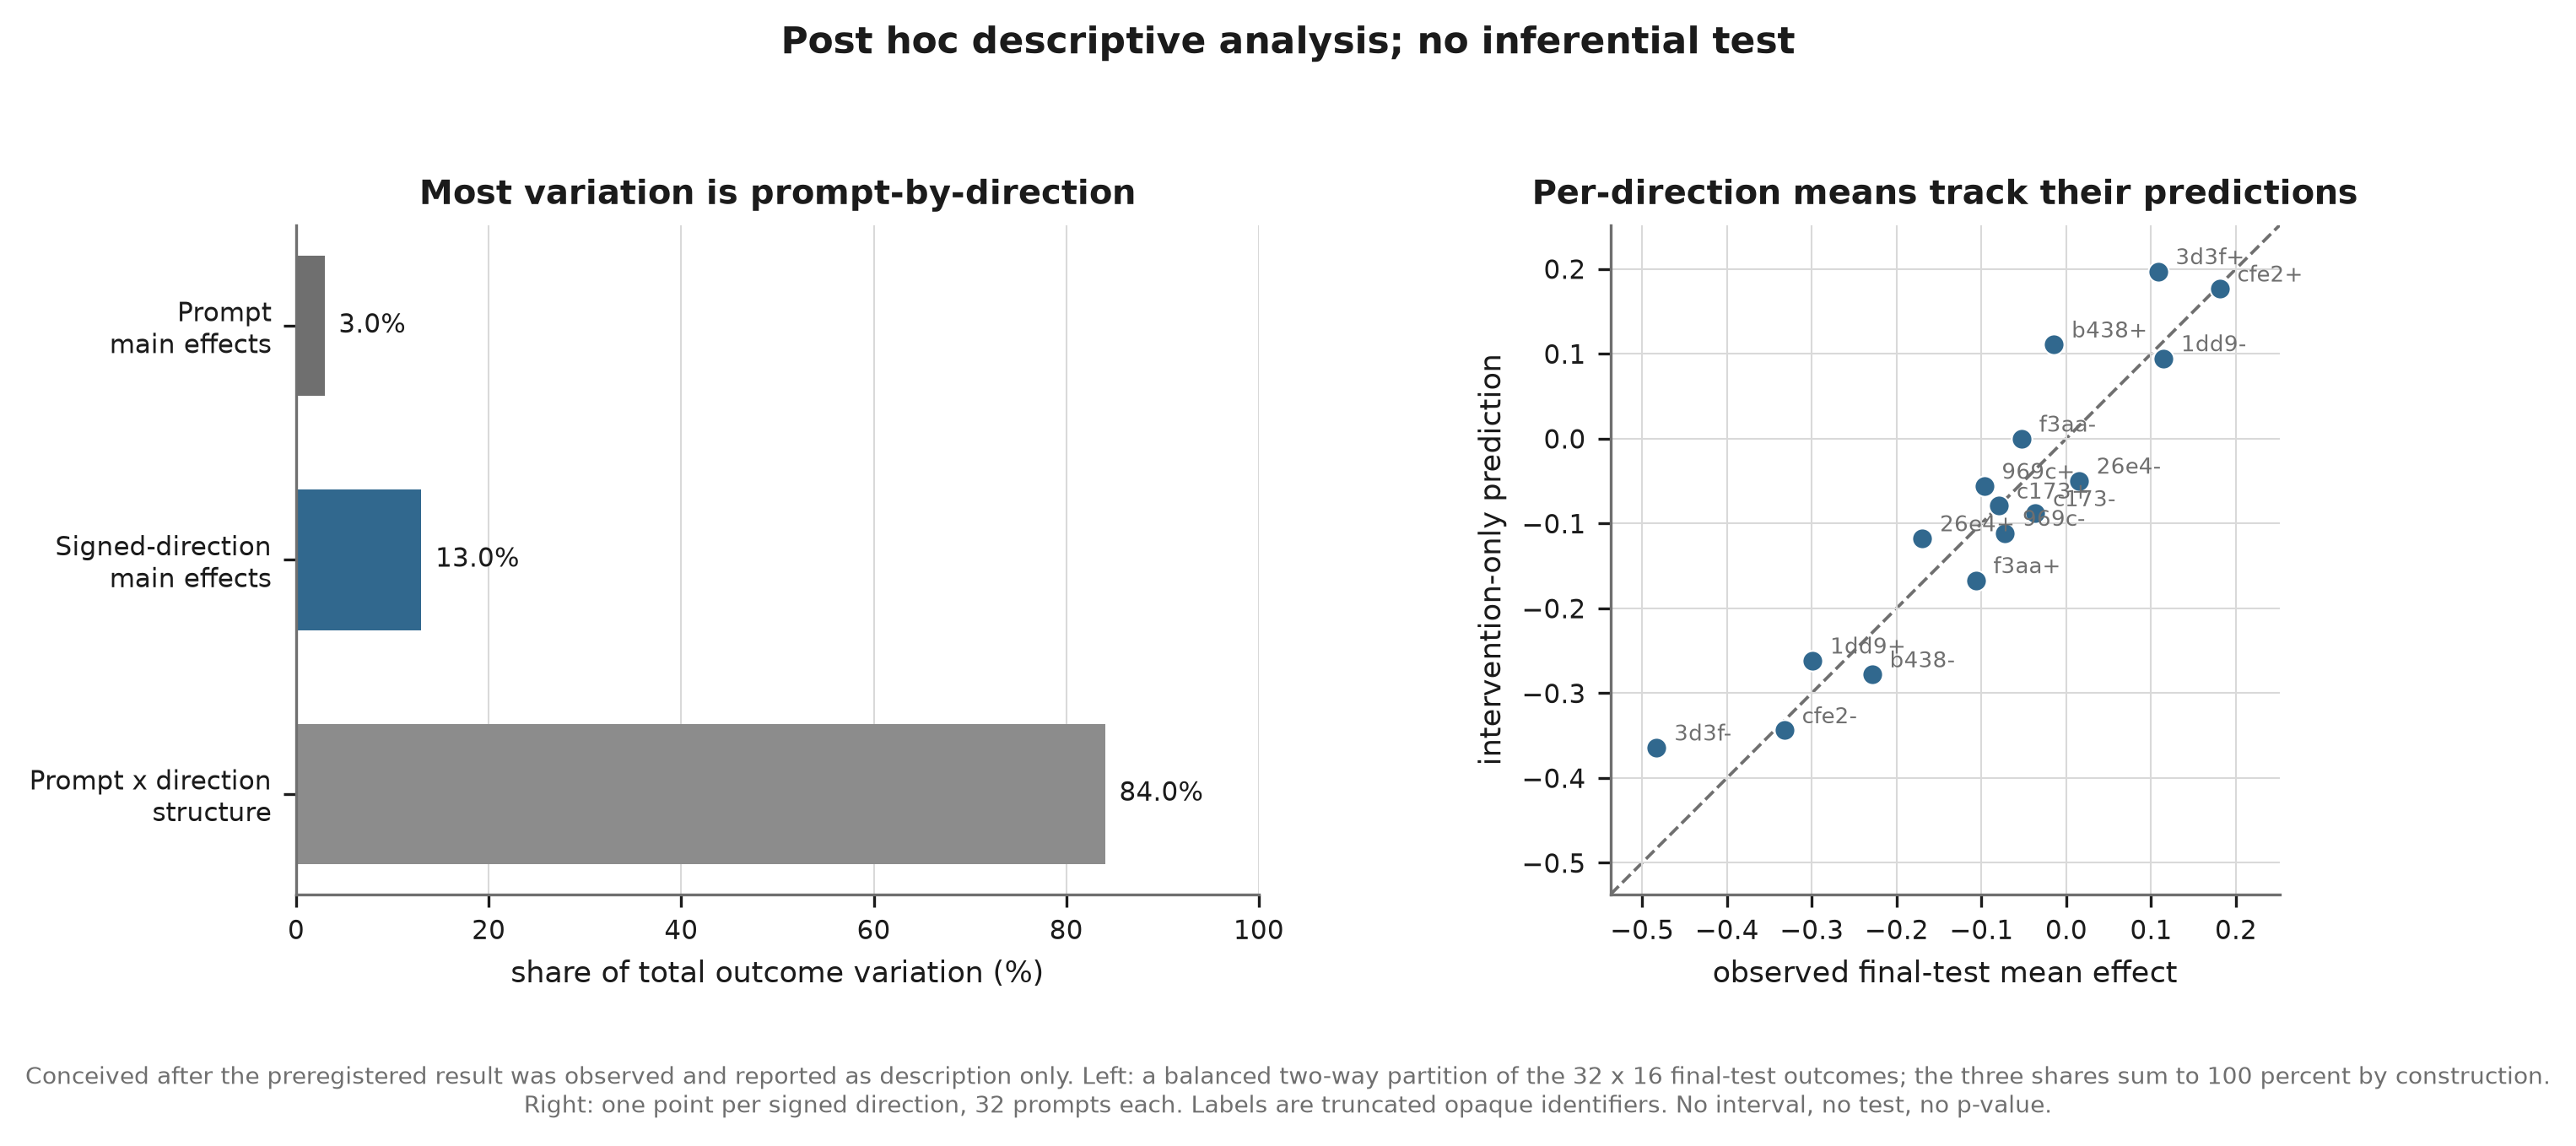
\includegraphics[width=0.96\textwidth]{figures/exploratory_direction_structure.png}
\caption{Post hoc descriptive analysis; no inferential test. Left: the partition above. Right: the
intervention-only prediction against the observed mean effect for each of the 16 signed directions,
labelled by truncated opaque identifier.}
\label{fig:decomposition}
\end{figure}

\section{Additional figures}
\label{app:figures-extra}

\begin{figure}[t]
\centering
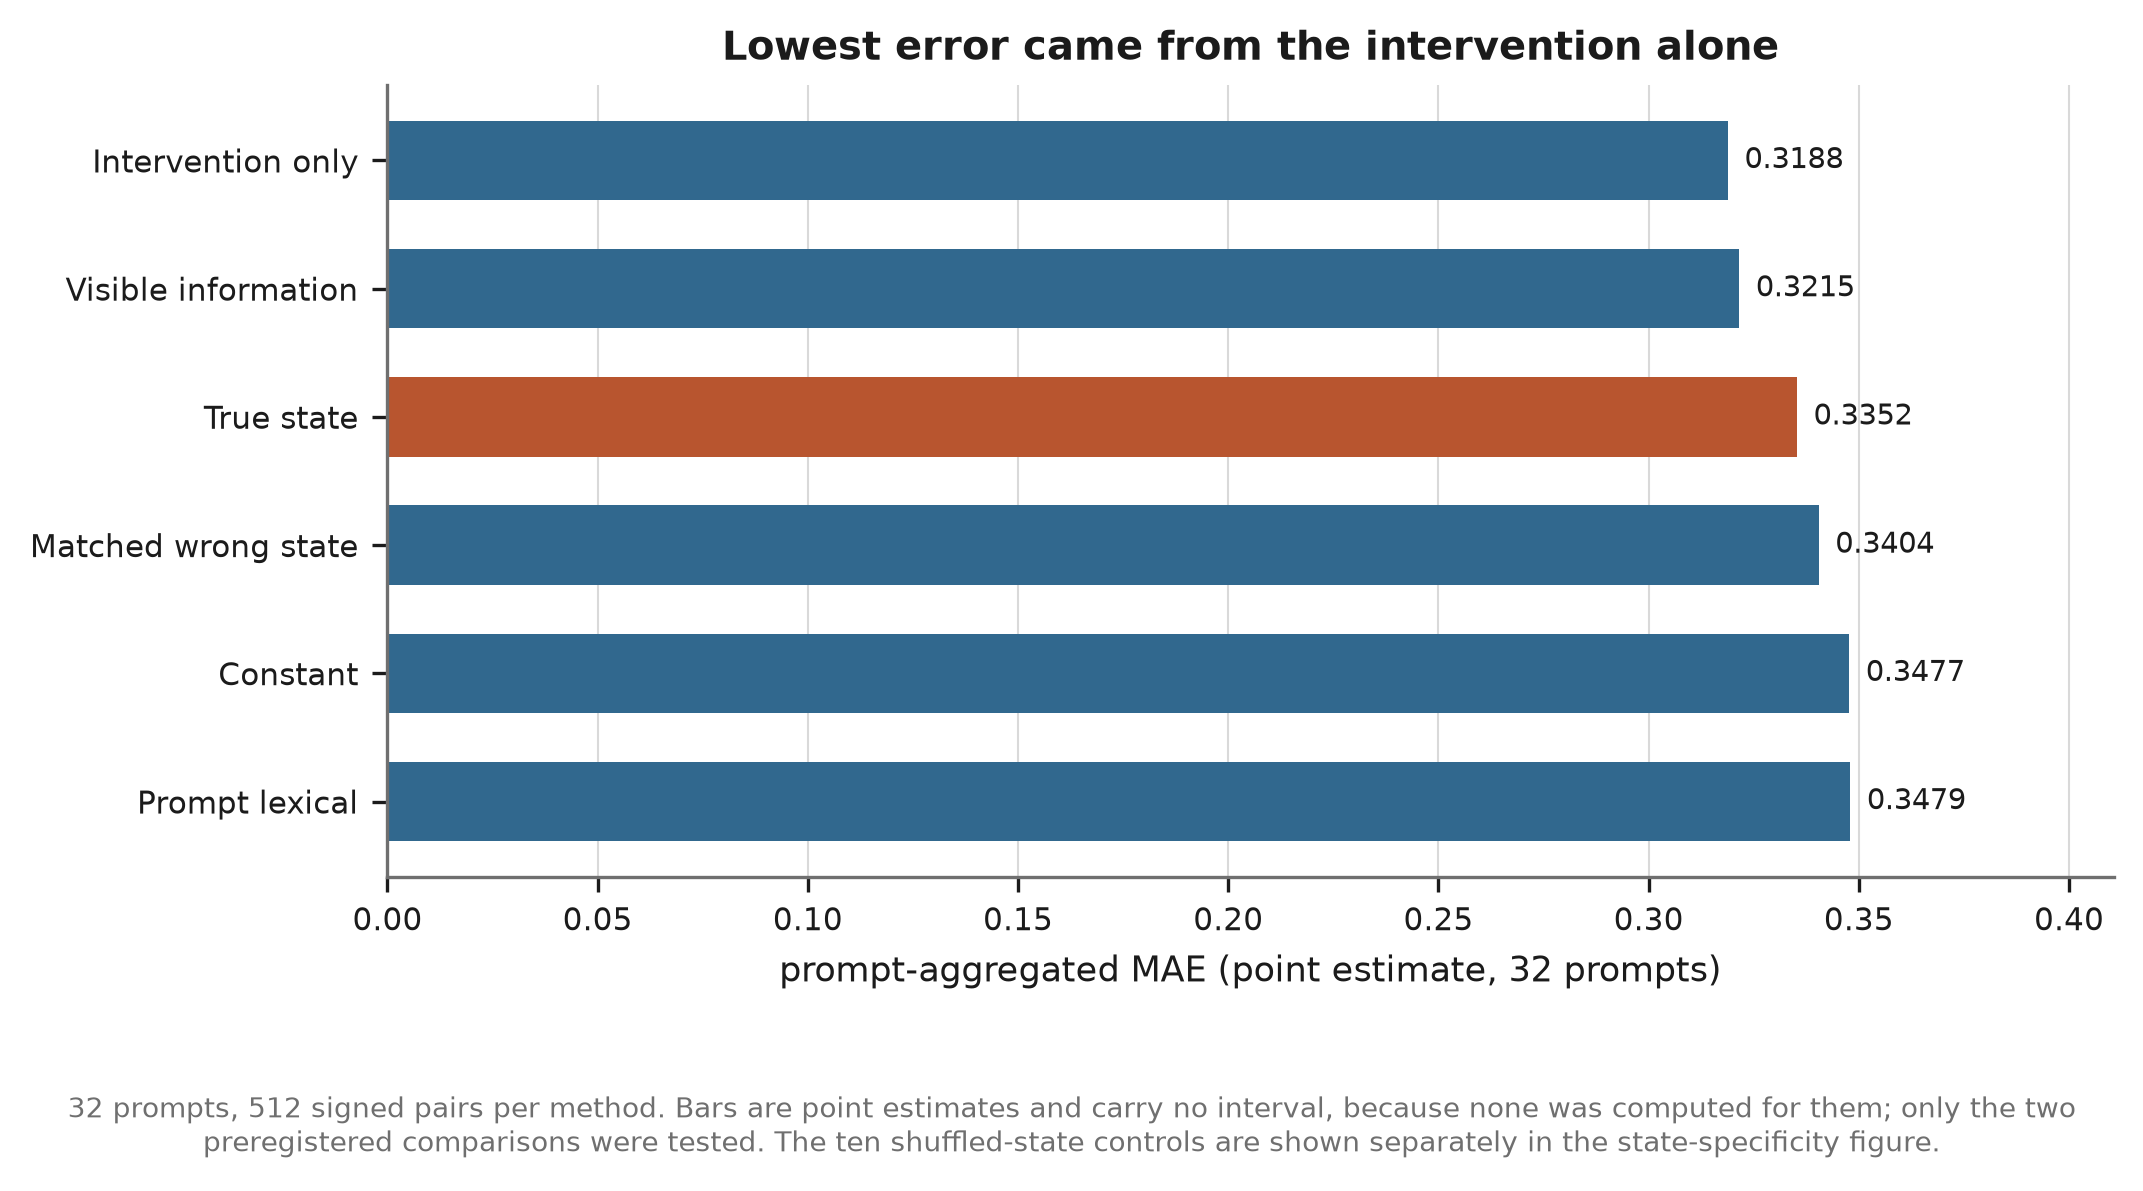
\includegraphics[width=0.78\textwidth]{figures/final_test_mae_by_method.png}
\caption{Prompt-aggregated MAE by method, sorted. Bars are point estimates and carry no
interval because none was computed for them. The ten shuffled-state controls appear separately in
Figure~\ref{fig:specificity}.}
\label{fig:mae}
\end{figure}

\begin{figure}[ht]
\centering
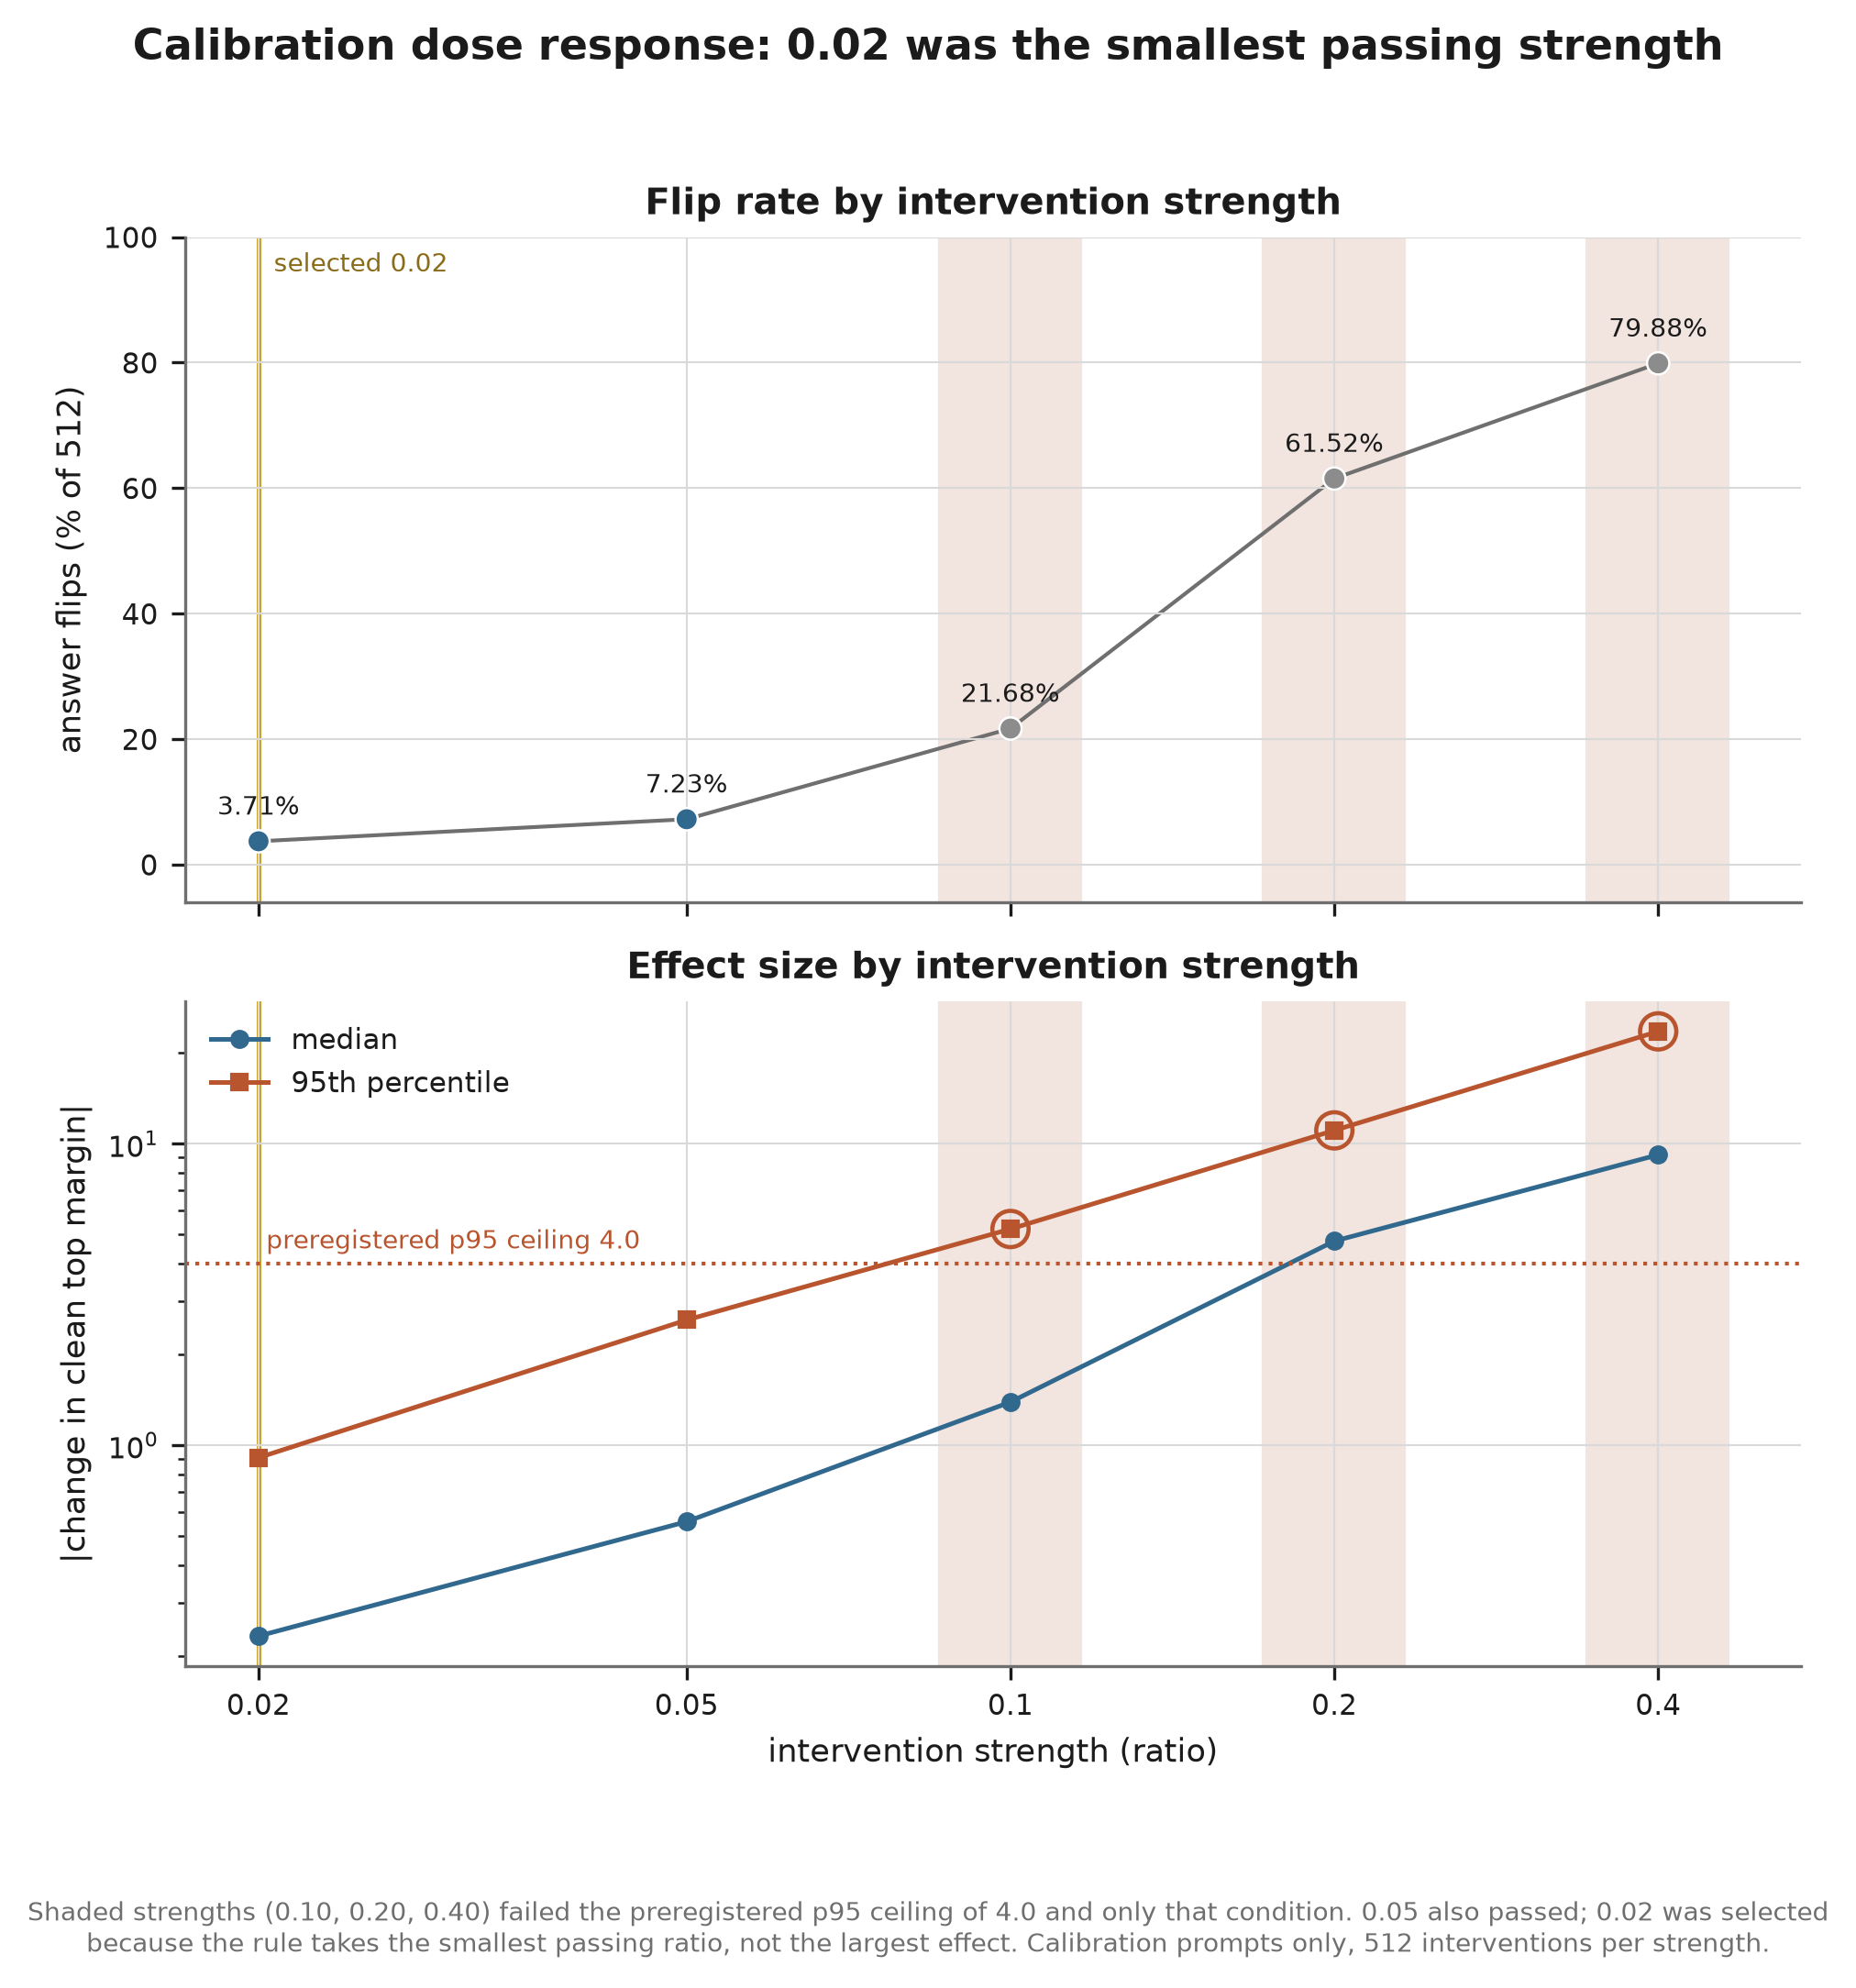
\includegraphics[width=0.62\textwidth]{figures/calibration_dose_response.png}
\caption{Calibration dose response. Shaded strengths failed the preregistered p95 ceiling, and only
that condition. 0.05 also passed; 0.02 was selected because the rule takes the smallest passing
ratio.}
\label{fig:dose}
\end{figure}

\begin{figure}[ht]
\centering
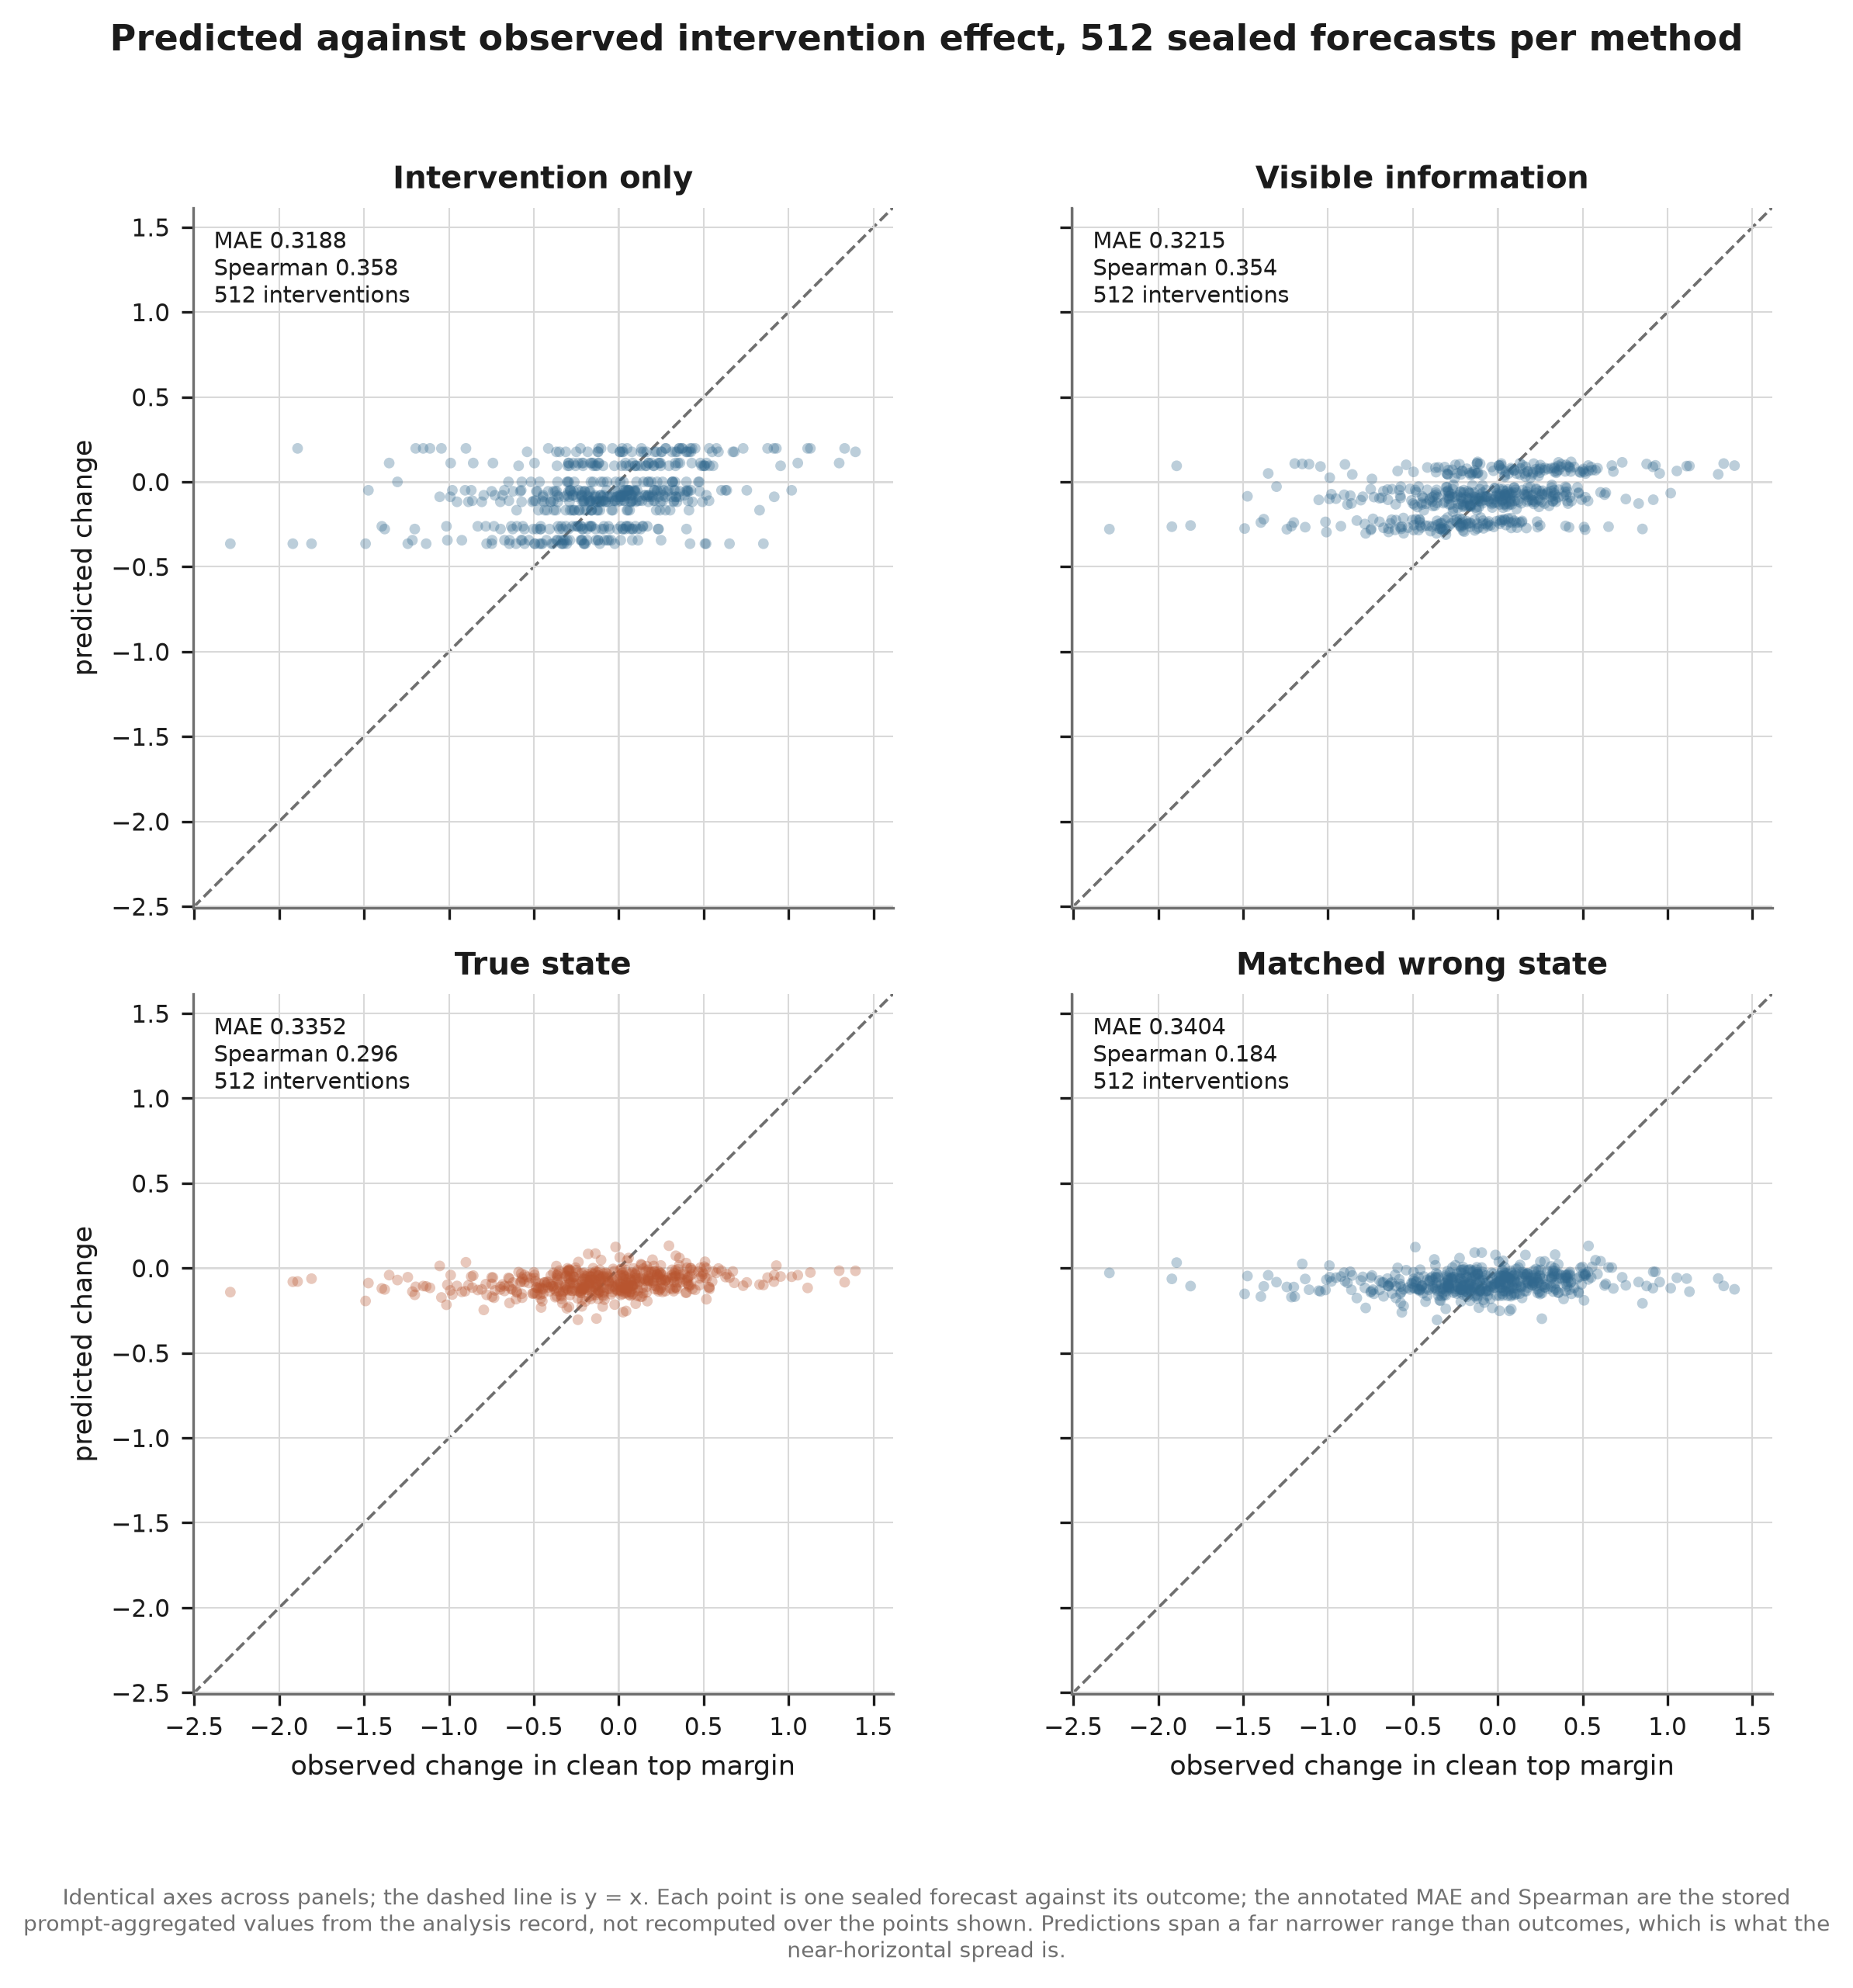
\includegraphics[width=0.70\textwidth]{figures/prediction_vs_observed.png}
\caption{Predicted against observed effect for the four ridge conditions, identical axes
throughout. The spread around $y=x$ is what the headline MAE summarises.}
\label{fig:scatter}
\end{figure}

\begin{figure}[ht]
\centering
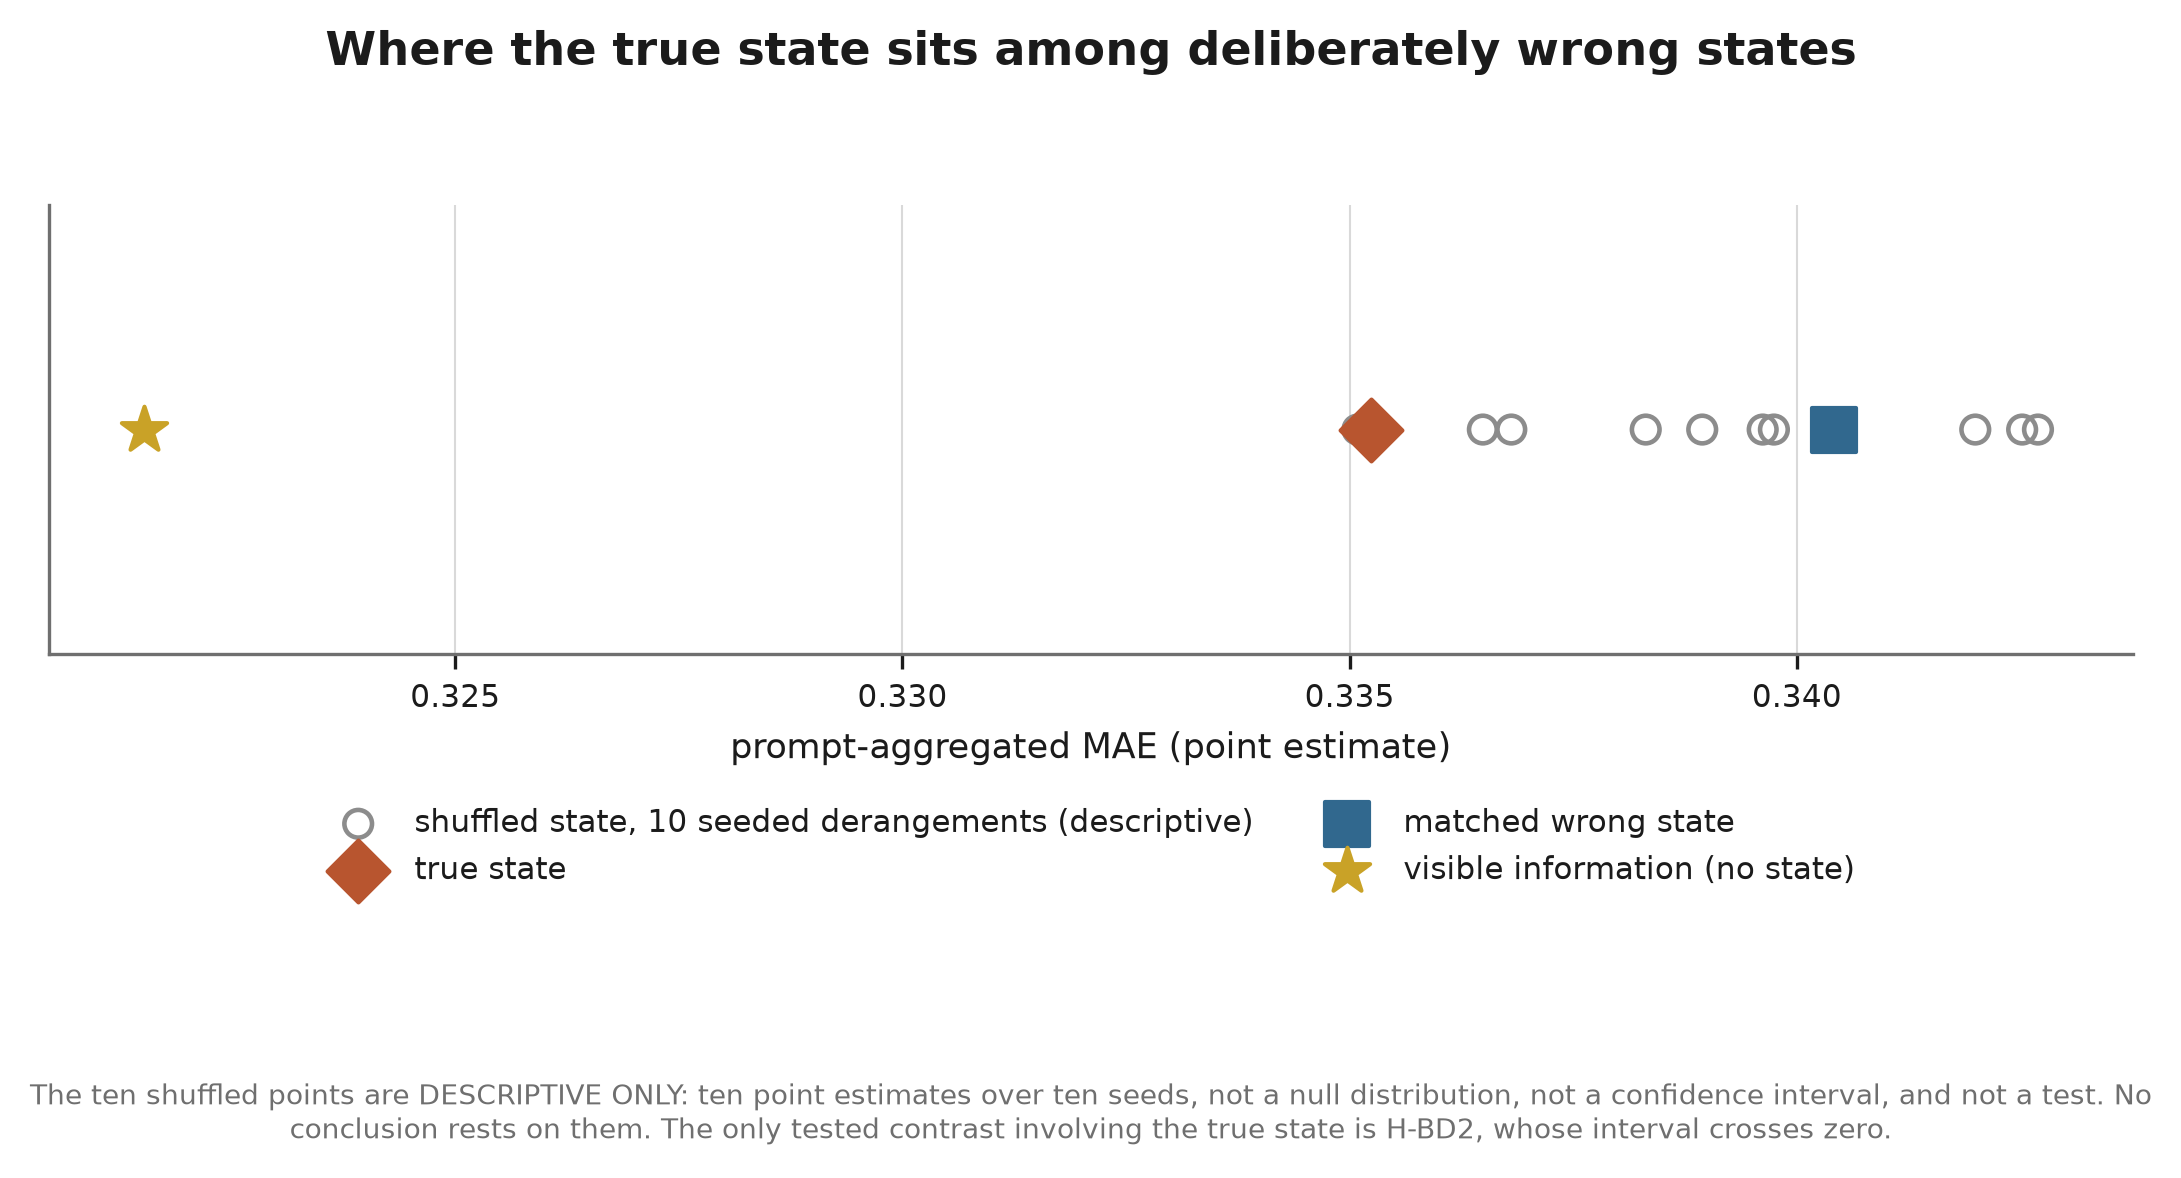
\includegraphics[width=0.82\textwidth]{figures/state_specificity.png}
\caption{The true-state score against the ten deranged-state controls. The controls are
descriptive: ten point estimates over ten seeds, not a null distribution and not a test.}
\label{fig:specificity}
\end{figure}

\begin{figure}[ht]
\centering
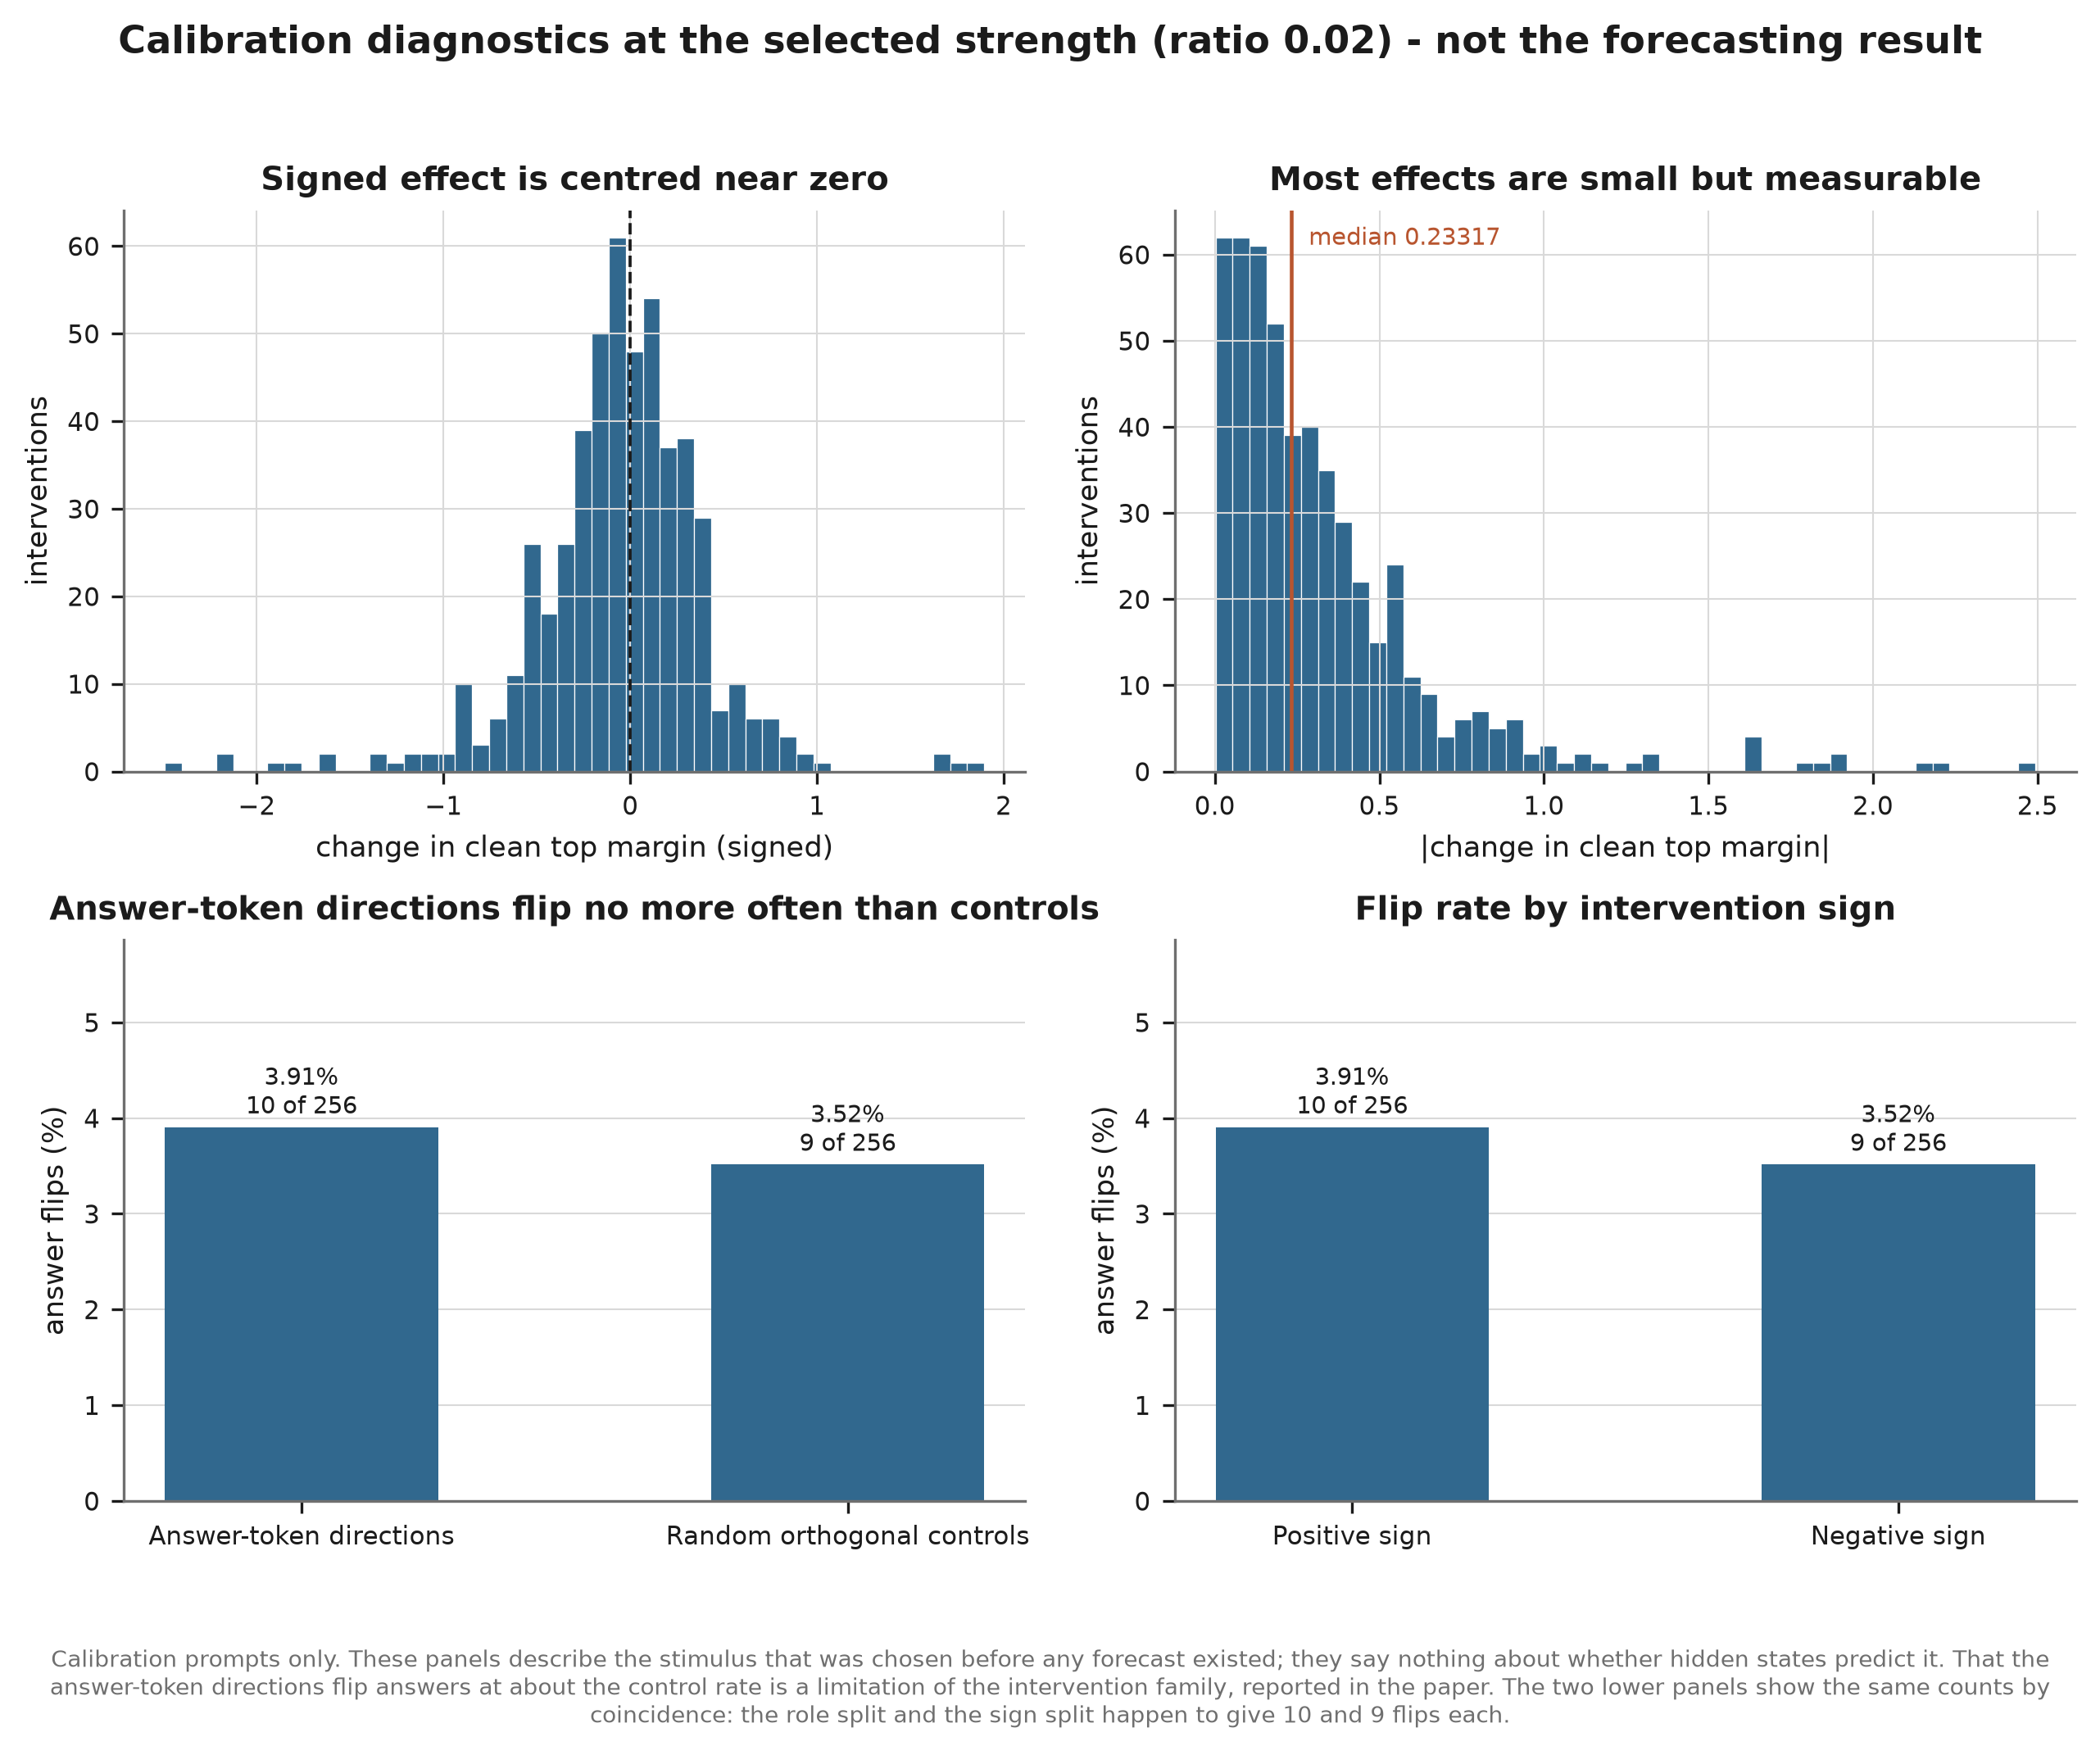
\includegraphics[width=0.80\textwidth]{figures/intervention_effects.png}
\caption{Calibration diagnostics at the selected strength, not the forecasting result. The lower
two panels show identical counts by coincidence.}
\label{fig:effects}
\end{figure}

\end{document}
